\documentclass[a4paper, 12pt]{article}
\usepackage[T2A]{fontenc}
\usepackage[utf8]{inputenc}
\usepackage[english,russian]{babel}
\usepackage{indentfirst}
\usepackage{hyperref}
\usepackage{fancyhdr}
\usepackage{lipsum}
\usepackage{geometry}
\usepackage{float}
\usepackage{chngcntr}
\usepackage{array}
\usepackage{textcomp}
\usepackage{graphicx}
\usepackage{amsmath, amssymb}
\usepackage[justification=centering]{caption}

\hypersetup{
    colorlinks=true,
    linkcolor=black,
    urlcolor=blue,
}
\urlstyle{same}

\makeatletter
\renewcommand{\@biblabel}[1]{#1.}
\makeatother
\newcommand{\bibref}[3]{#2 \hyperlink{#1}{\color{blue}(#3)}}

\graphicspath{ {./images/} }

\newcolumntype{M}[1]{>{\centering\arraybackslash}m{#1}}
\counterwithin{table}{section}
\counterwithin{figure}{section}
\counterwithin{equation}{section}

\geometry{left=2.5cm}
\geometry{right=1.5cm}
\geometry{top=1.5cm}
\geometry{bottom=1.5cm}
\renewcommand{\baselinestretch}{1.5}

\pagestyle{fancy}
\fancyhead{}
\fancyfoot{}
\fancyfoot[R]{\thepage}

\DeclareMathOperator*{\argmin}{argmin}

\begin{document}

\thispagestyle{empty}

\textbf{
\begin{center}
    Федеральное государственное автономное образовательное \\
    учреждение высшего образования \\
    «Национальный исследовательский университет \\
    «Высшая школа экономики»» \\
\end{center}
\begin{center}
    Факультет компьютерных наук \\
    Основная образовательная программа \\
    Прикладная математика и информатика
\end{center}
\vspace{15pt}
\begin{center}
    \Large
    КУРСОВАЯ РАБОТА \\
    (Исследовательский проект) \\
    Исследование процессов убывания площади групп солнечных пятен
\end{center}
}

\vspace{6pt}
\noindent
\textbf{Выполнил студент группы 171, 3 курса, \\
Садртдинов Ильдус Рустемович \\
}

\vspace{6pt}
\noindent
\textbf{Руководитель КР: \\
Д. ф.-м. н., Профессор ДБДИП, Шаповал Александр Борисович
}

\vspace{\fill}
\begin{center}
\textbf{Москва 2020}
\end{center}
\newpage

\tableofcontents
\newpage

\section{Аннотация}

\subsection{Аннотация}

На сегодняшний день процессы убывания площади солнечных пятен исследованы не полностью, в том числе, не существует единого мнения о том, как скорость убывания зависит от площади и как площадь уменьшается с течением времени. В этой работе рассматривается подход, основанный на методах машинного обучения. Основная идея - приблизить закон убывания площади некоторой регрессионной моделью, обучаемой на доступных данных. Результатом работы является алгоритм, предсказывающий площади солнечных пятен, который в дальнейшем можно применять для других задач изучения солнечной активности.

\subsection{Abstract}

The processes of sunspot area decay still are not fully understood. Furthermore, there is no consensus on decay rate formula and area decay law. This study focuses on machine learning application to this problem. The main idea is to approximate the decay law with a regression model trained on the available data. The significant result of the study is an area prediction algorithm that might be useful for different solar activity problems.

\subsection{Список ключевых слов}

Солнечные пятна, солнечная активность, машинное обучение, регрессионная модель, скорость убывания площади, логнормальное распределение.

\newpage

\section{Введение}

Исходный код работы доступен на \href{https://github.com/isadrtdinov/Solar-Activity}{GitHub}

Солнечные пятна – это темные области на поверхности Солнца, их существование объясняется выходом сильных магнитных полей в солнечную фотосферу. По этой причине солнечные пятна тесно связаны с понятием солнечной активности. На сегодняшний день солнечные пятна являются объектом интереса исследователей, поскольку наблюдения за ними ведутся на протяжении последних нескольких веков, в то время как более современные методы исследования магнитного поля Солнца появились только в XX веке. Типичный цикл солнечной активности длится приблизительно 11 лет, поэтому изучение солнечных пятен позволяет использовать большие объемы данных для анализа и, как следствие, охватить большее число солнечных циклов.

Эта работа посвящена изучению отдельных групп солнечных пятен, а именно, изменению площади группы с течением времени ее жизни (эта величина традиционно измеряется в миллионных долях солнечного диска - $\mu$Hem). Большинство групп пятен имеют относительно небольшую площадь (менее 100 $\mu$Hem) и существуют на поверхности Солнца около 2-3 дней. Интерес представляют группы с большей площадью (порядка нескольких сотен $\mu$Hem), обладающие большим временем жизни. Как правило, такие группы быстро дорастают до максимума площади, а в течение всего оставшегося времени жизни площадь группы убывает. Основная цель этого исследования – выявление закономерностей убывания площади долгоживущих групп солнечных пятен.

\subsection{Основные идеи исследования}

Приходится констатировать, что наблюдаемые данные о площади солнечных пятен сильно зашумлены. Это обстоятельство связано как с несовершенством наблюдений за Солнцем, так и с самим поведением солнечных пятен. Как будет показано в дальнейшем, сильнее всего этот эффект влияет на группы пятен небольшой площади, а также на группы пятен, расположенные на периферии солнечного диска. Таким образом, исходные данные нуждаются в дополнительной фильтрации, прежде чем они могут быть использованы для обучения регрессионных моделей.

В ходе этой работы разработано несколько моделей, предсказывающих площадь группы пятен по показателям площади за несколько предыдущих наблюдений. Менее формально, идея всего исследования описывается так: можно аппроксимировать поведение групп солнечных пятен с помощью обученной модели, а затем выводить законы убывания площади, подменяя зашумленные исходные данные на предсказания модели. Более строго, все исследование можно разбить на несколько смысловых составляющих:

\begin{enumerate}
    \item Предварительная фильтрация данных, их подготовка к обучению моделей
    \item Рассмотрение нескольких моделей для предсказания площади групп пятен, отбор наиболее подходящей.
    \item Применение наилучшей модели для анализа скорости убывания площади.
\end{enumerate}

Отбор моделей в данном случае является нетривиальной задачей, поскольку необходимо принимать во внимание не только количественные показатели (ошибка алгоритма на тестовой выборке), но и некоторые качественные показатели (такие как, например, распределение скорости убывания площади). Разумным подходом кажется сравнивать модели по количественным показателям, отбраковывать те, что показывают себя хуже остальных, а затем проверять качественные показатели на наиболее удачных моделях. В конечном итоге, обученная модель будет применяться для вывода закона убывания площади групп пятен.

\section{Обзор литературы}

На сегодняшний день проведено несколько исследований, посвященных убыванию площадей солнечных пятен. В этих работах особое место уделяется величине, называемой скоростью убывания площади (англ. decrease rate). В статье \bibref{petrovay}{Petrovay K., Van Driel-Gesztelyi L.}{1997} выводится эмпирическая зависимость скорости убывания площади от радиуса группы; соотношение, полученное авторами, имеет вид $D \propto \frac{r}{r_0}$, где $D$ - средняя скорость убывания площади, $r$ - текущий радиус группы пятен, а $r_0$ - ее максимальный радиус. Результаты, полученные авторами, опровергают более ранние исследования, согласно которым скорость убывания площади является постоянной (\bibref{bumba}{Bumba V.}{1963}).

Другая релевантная работа описана в статье \bibref{hathaway}{Hathaway D.H., Choudhary D.P.}{2008}. В этом исследовании авторы разбивают группы пятен по площади на несколько корзин и изучают их по отдельности. В итоге, они приходят к следующему выводу: при площади групп от 35 $\mu$Hem до приблизительно 1000 $\mu$Hem средняя скорость убывания линейно возрастает по площади, а для площадей, больших 1000 $\mu$Hem, средняя скорость убывания становится близка к константе. При этом, авторы устанавливают, что скорость убывания имеет логнормальное распределение.

Также важно отметить метод, с помощью которого авторы избавлялись от выбросов в данных. Прежде всего они исключили из рассмотрения те наблюдения, которые отстоят от центрального меридиана Солнца больше, чем на $60^{\circ}$. Поскольку периферия солнечного диска с Земли видна под углом, то группа пятен наблюдается в некоторой проекции, поэтому площади корректируются в соответствии с углом наблюдения. Исключение периферийных наблюдений позволяет устранить группы пятен, для которых площадь была скорректирована сильно (ввиду большого угла наблюдения). Кроме того, авторы не рассматривают группы с площадями, меньшими 35 $\mu$Hem, так как для маленьких пятен измерения имеют меньшую точность. Статья фокусируется на убывании площадей, поэтому в качестве выборки рассматриваются наблюдения, идущие после максимума площади группы. Также, для исключения шумовой компоненты данных, в выборку попадают только те фрагменты истории групп, в которых площадь убывала последние три дня до наблюдения. В этой работе предлагается использовать сходный метод для фильтрации данных.

Таким образом, на сегодняшний день известны несколько эмпирических зависимостей для скорости убывания площади. В этой работе предлагается использовать методы машинного обучения для подтверждения или опровержения этих формул.

\section{Обзор данных}

\subsection{Данные и сопряженные с ними проблемы}

Используемые в работе данные были предоставлены Гринвичской королевской обсерваторией \bibref{rgo}{}{Royal Observatory, Greenwich} и содержат ежедневные записи о наблюдаемых солнечных пятнах с 1874 по 1974 год. Одна запись содержит время и дату наблюдения, номер группы, а также ее координаты (широту и долготу относительного центрального меридиана в градусах) и площадь (наблюдаемую и скорректированную с учетом ракурса наблюдения), см. таблицу 4.1.

\vspace{0.75cm}

\begin{table}[H]
\centering

\begin{tabular}{|M{2.5cm}|M{2cm}|M{2.5cm}|M{2.4cm}|M{2.2cm}|M{2.2cm}|}
\hline
Время наблюдения & № группы & Наблюдаемая площадь ($\mu$Hem) & Скорректир. площадь ($\mu$Hem) & Широта (\textdegree) & Долгота (\textdegree) \\
\hline
1874-05-09 11:55:40 & 8600 & 639.0 & 378.0 & 7.4 & -30.7 \\
\hline
\end{tabular}

\caption{\label{tab:table-name} Пример описания одного наблюдения за группой пятен.}
\end{table}

Работа с данными по солнечным пятнам сопряжена с несколькими проблемами, усложняющими анализ. Как было упомянуто выше, точность измерения площадей маленьких и периферийных групп пятен не высока, кроме того, на площади сильно влияет шумовая компонента, что сильно затрудняет выделение трендов (особенно заметен этот эффект для пятен небольшой площади).

Также, существует проблема, связанная с вращением Солнца вокруг своей оси: дело в том, что пятна обращаются вместе с Солнцем, поэтому зачастую группы пятен скрываются от наблюдателя за горизонтом (точнее говоря, за западным лимбом Солнца), оказываясь на невидимой с Земли стороне. Период обращения Солнца вокруг своей оси составляет около 27-28 дней, поэтому в базе данных практически отсутствуют записи о группах пятен, существовавших более 14 дней (половина периода обращения Солнца). Такая же проблема сопряжена с появлением новых групп пятен: если группа рождается на периферии солнечного диска, то нельзя с уверенностью сказать, образовалось ли новая группа, или же группа пришла с невидимой стороны вместе с Солнцем. Эту проблему легко вычленить, если нарисовать распределение времени жизни групп пятен на основе исходных данных (рис. 4.1).

\begin{figure}[H]
    \centering
    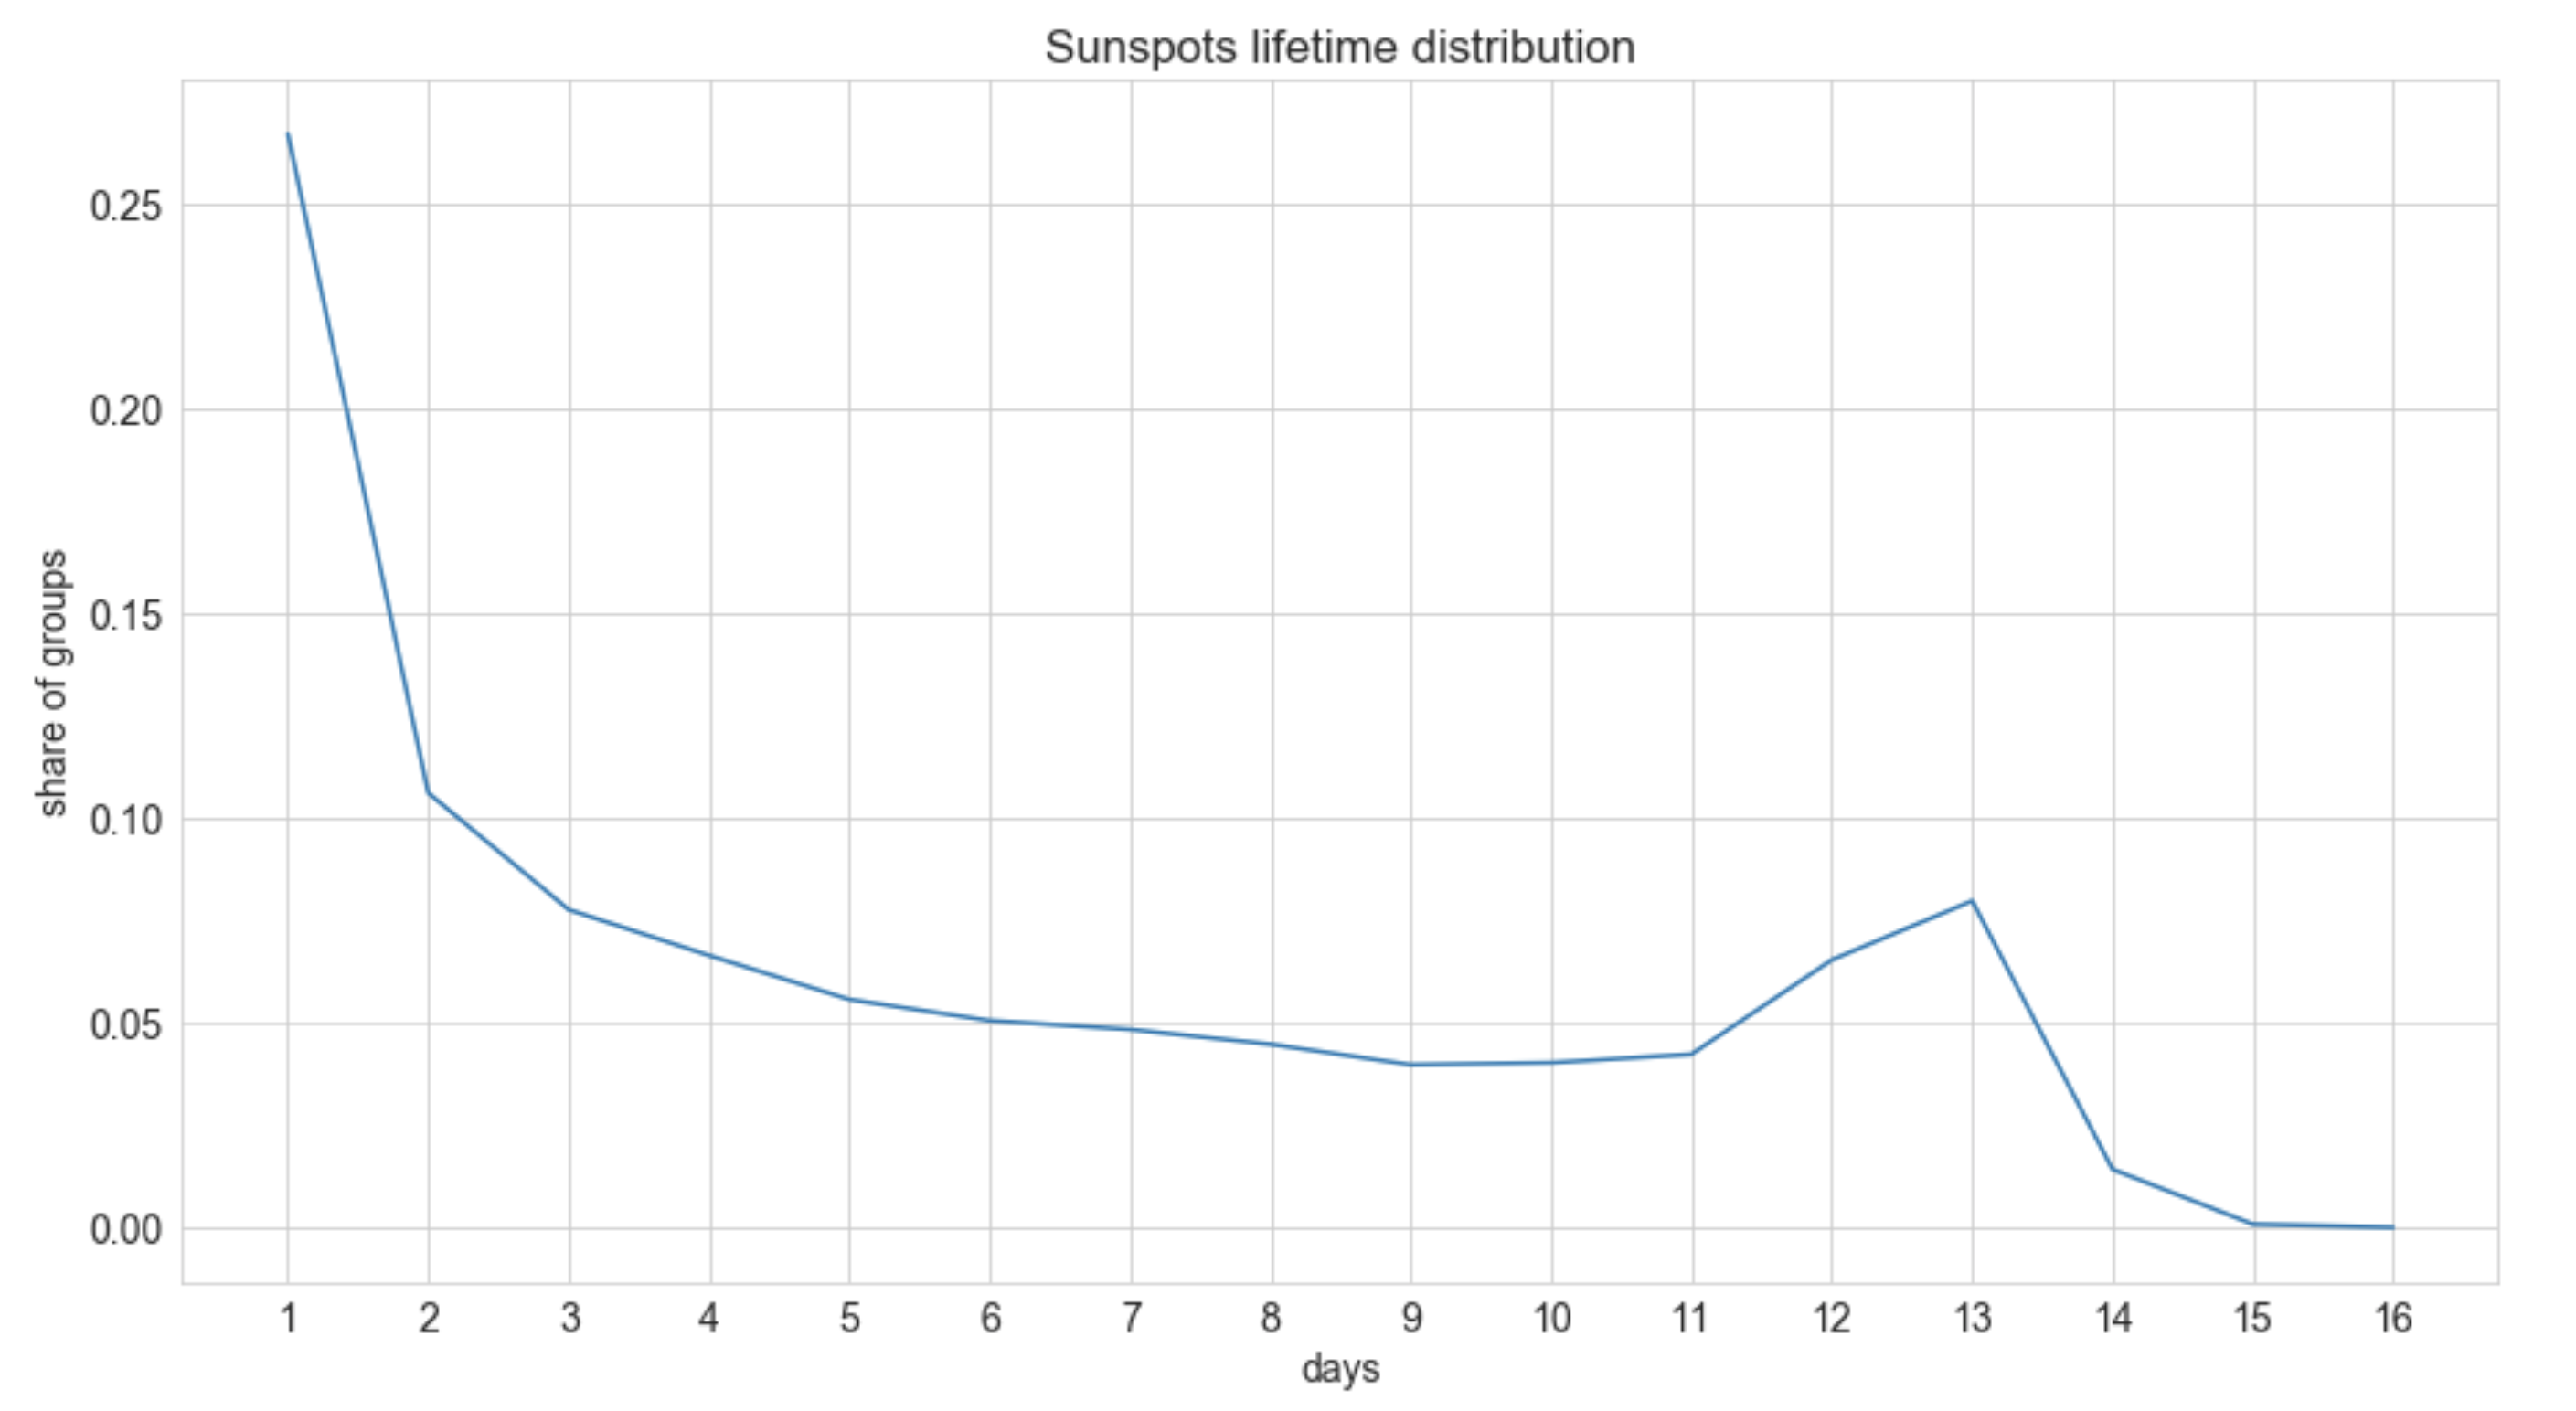
\includegraphics[width=17cm]{init_lifetime_distr.png}
    \caption{Распределение времени жизни групп солнечных пятен на основе исходных данных. По горизонтальной оси отложено время жизни группы в днях, по вертикали - доля групп, имеющих соответствующее время жизни.}
    \label{fig:my_label}
\end{figure}{}

На графике четко виден пик на 13-ый день, однако его существование объясняется не естественным поведением солнечных пятен, а несовершенством наблюдений за Солнцем. Поскольку часть пятен скрывается за горизонтом, то их полная история наблюдений оказывается недоступна, что и приводит к образованию пика.

\subsection{Фильтрация данных}

Необходимость фильтрации данных можно диагностировать непосредственно. Этот раздел посвящен нескольким графикам, которые наглядно демонстрируют мотивацию фильтровать данные, а также аргументируют тот метод фильтрации, что будет использоваться для формирования обучающей выборки. 

\begin{figure}[H]
    \centering
    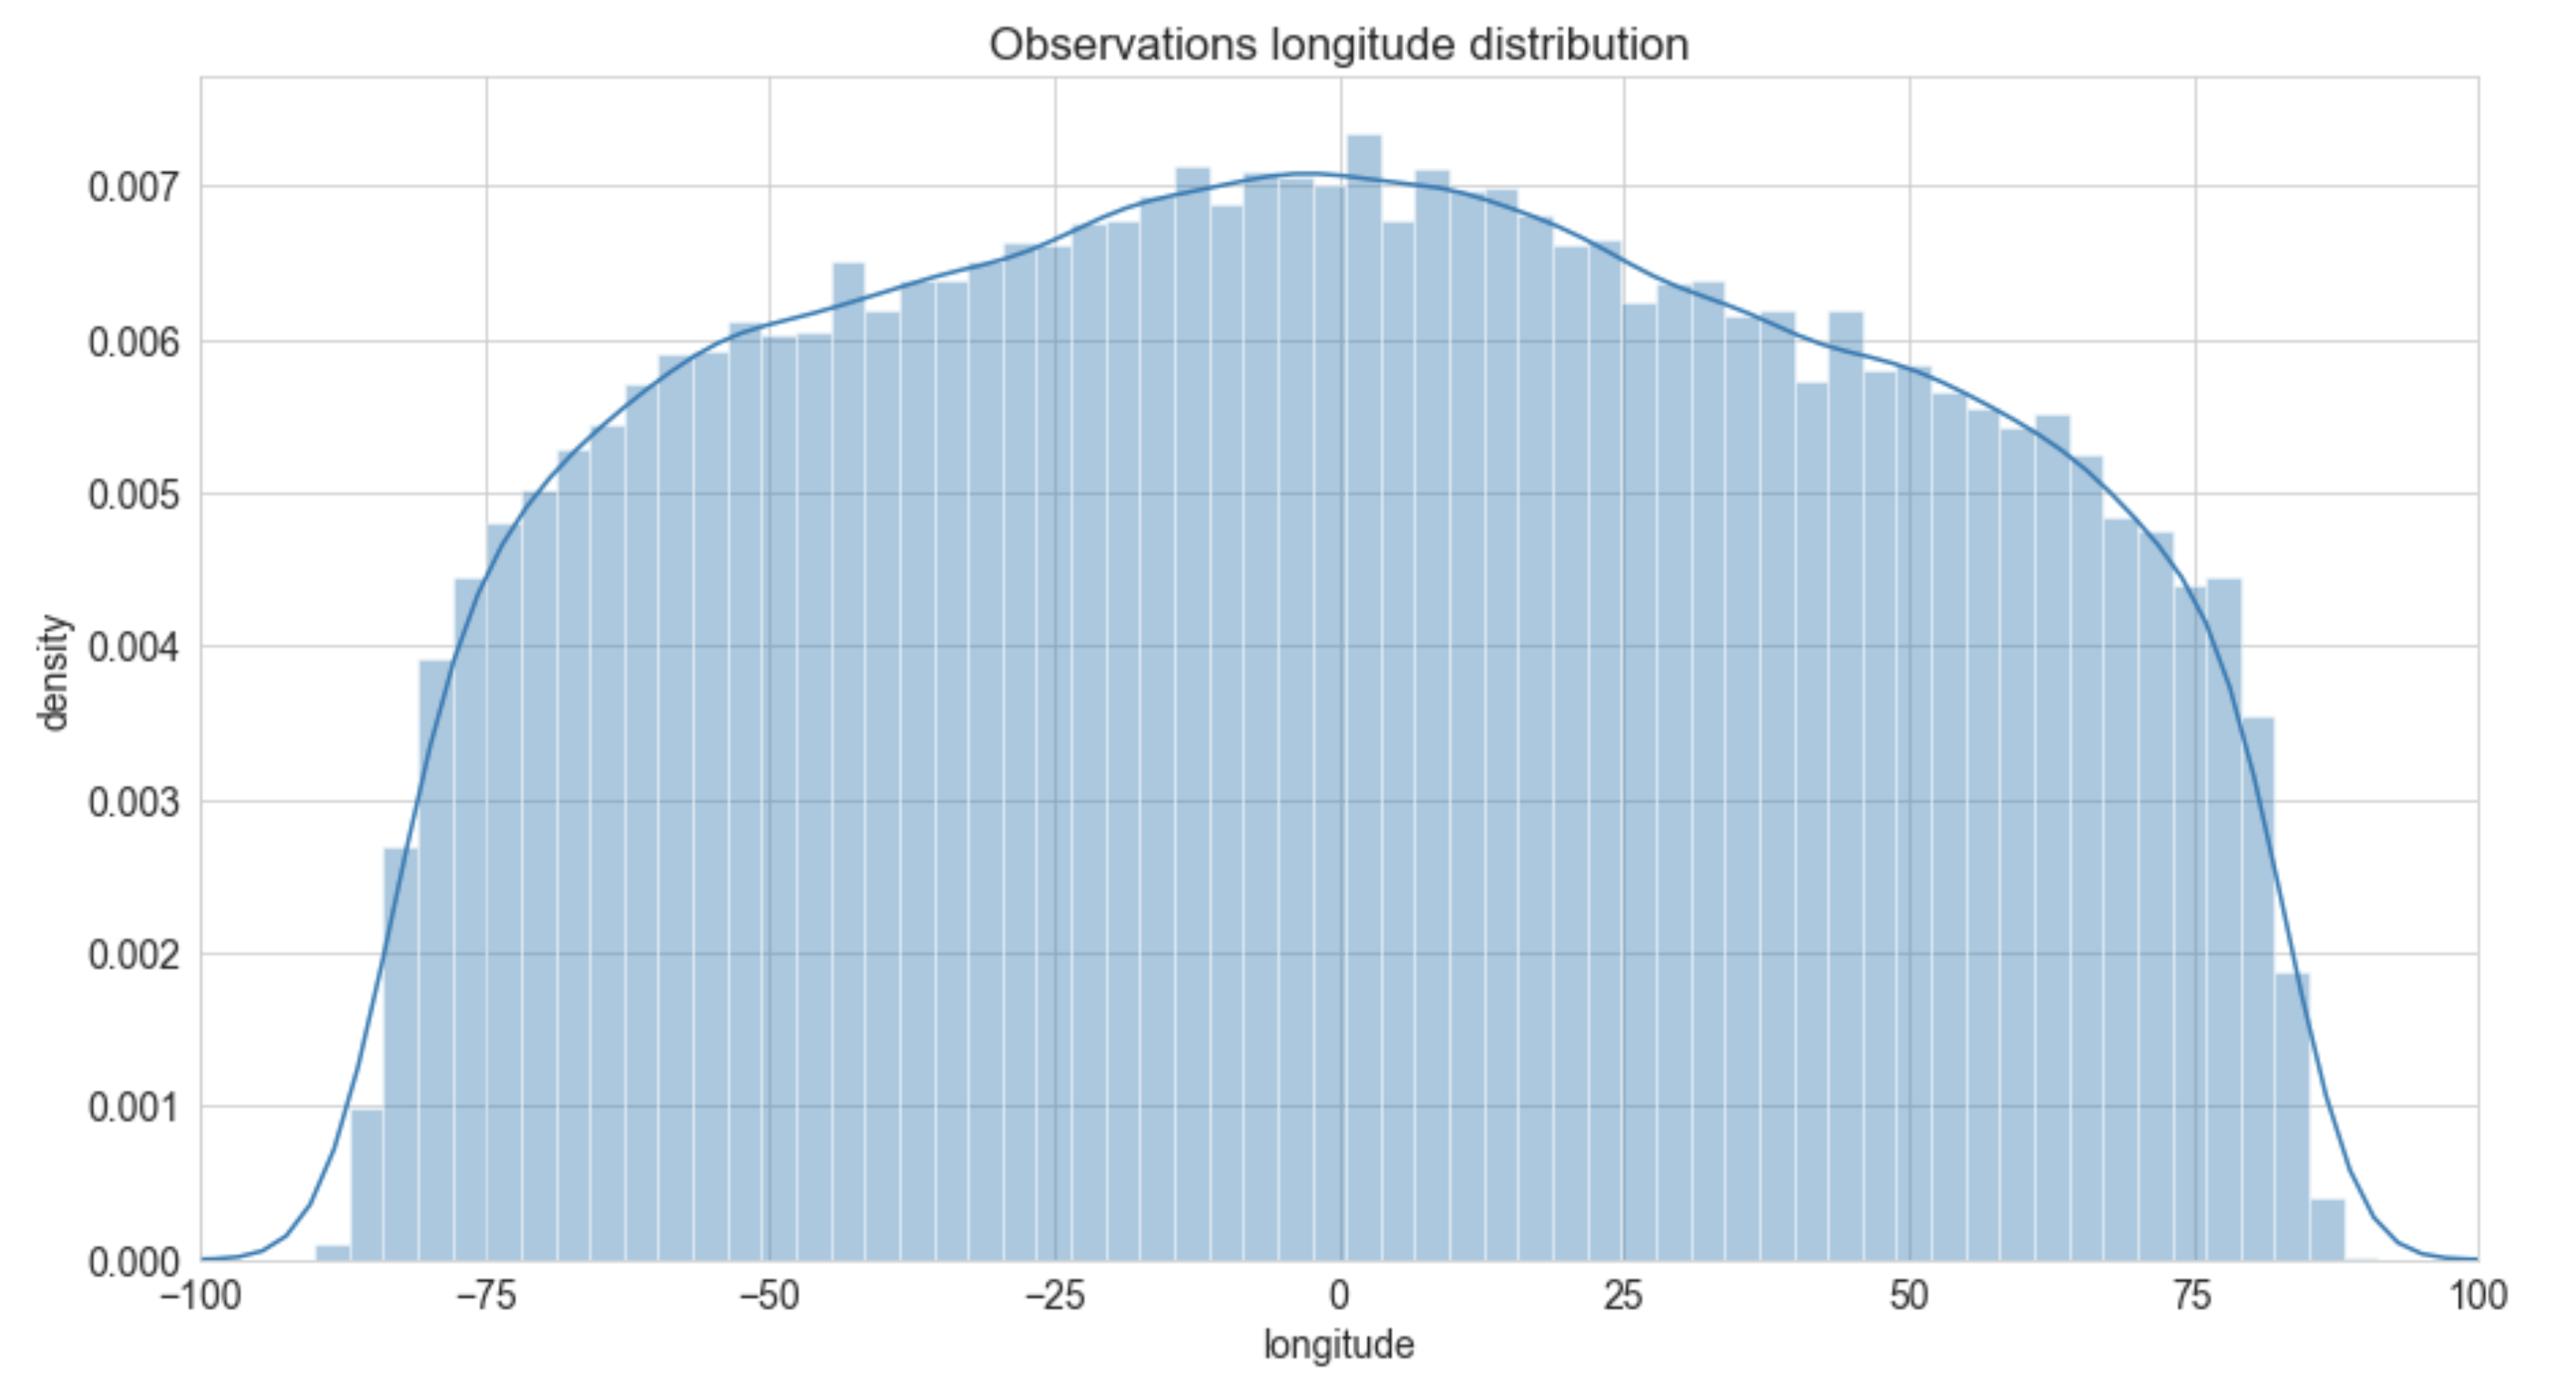
\includegraphics[width=17cm]{longitude_distr.png}
    \caption{Плотность распределения долгот наблюдений за группами пятен.}
    \label{fig:my_label}
\end{figure}{}

На рис. 4.2 изображена плотность распределения долгот наблюдений за группами солнечных пятен. Куполообразный вид распределения является свидетелем того факта, что периферийные наблюдения искажаются. Неформально это объясняется тем, что видимость вдоль края солнечного диска хуже. Этот эффект приводит к тому, что плотность рассматриваемого распределения становится больше при приближении к центральному меридиану ($0^\circ$) и уменьшается при приближении к краям диска ($-90^\circ, 90^\circ$).

Другой график мотивирует фильтрацию по минимальной площади. Как показано на рис. 4.1, большинство групп пятен существует не более 3-4 дней, поэтому они не представляют интереса для изучения долгосрочного убывания площади. Как правило, такие группы пятен имеют относительно небольшую плошадь (менее 100 $\mu$Hem), а потому исключение наблюдений за маленькими группами не принесет большого ущерба полноте выборки. Кроме того, как утверждают авторы в \bibref{hathaway}{Hathaway D.H., Choudhary D.P.}{2008}, на маленькие группы пятен сильнее влияет ошибка измерения, что непременно увеличивает шумовую компоненту в данных, задействуемых при обучении моделей, а это может пагубно сказаться на их итоговом качестве.

\begin{figure}[H]
    \centering
    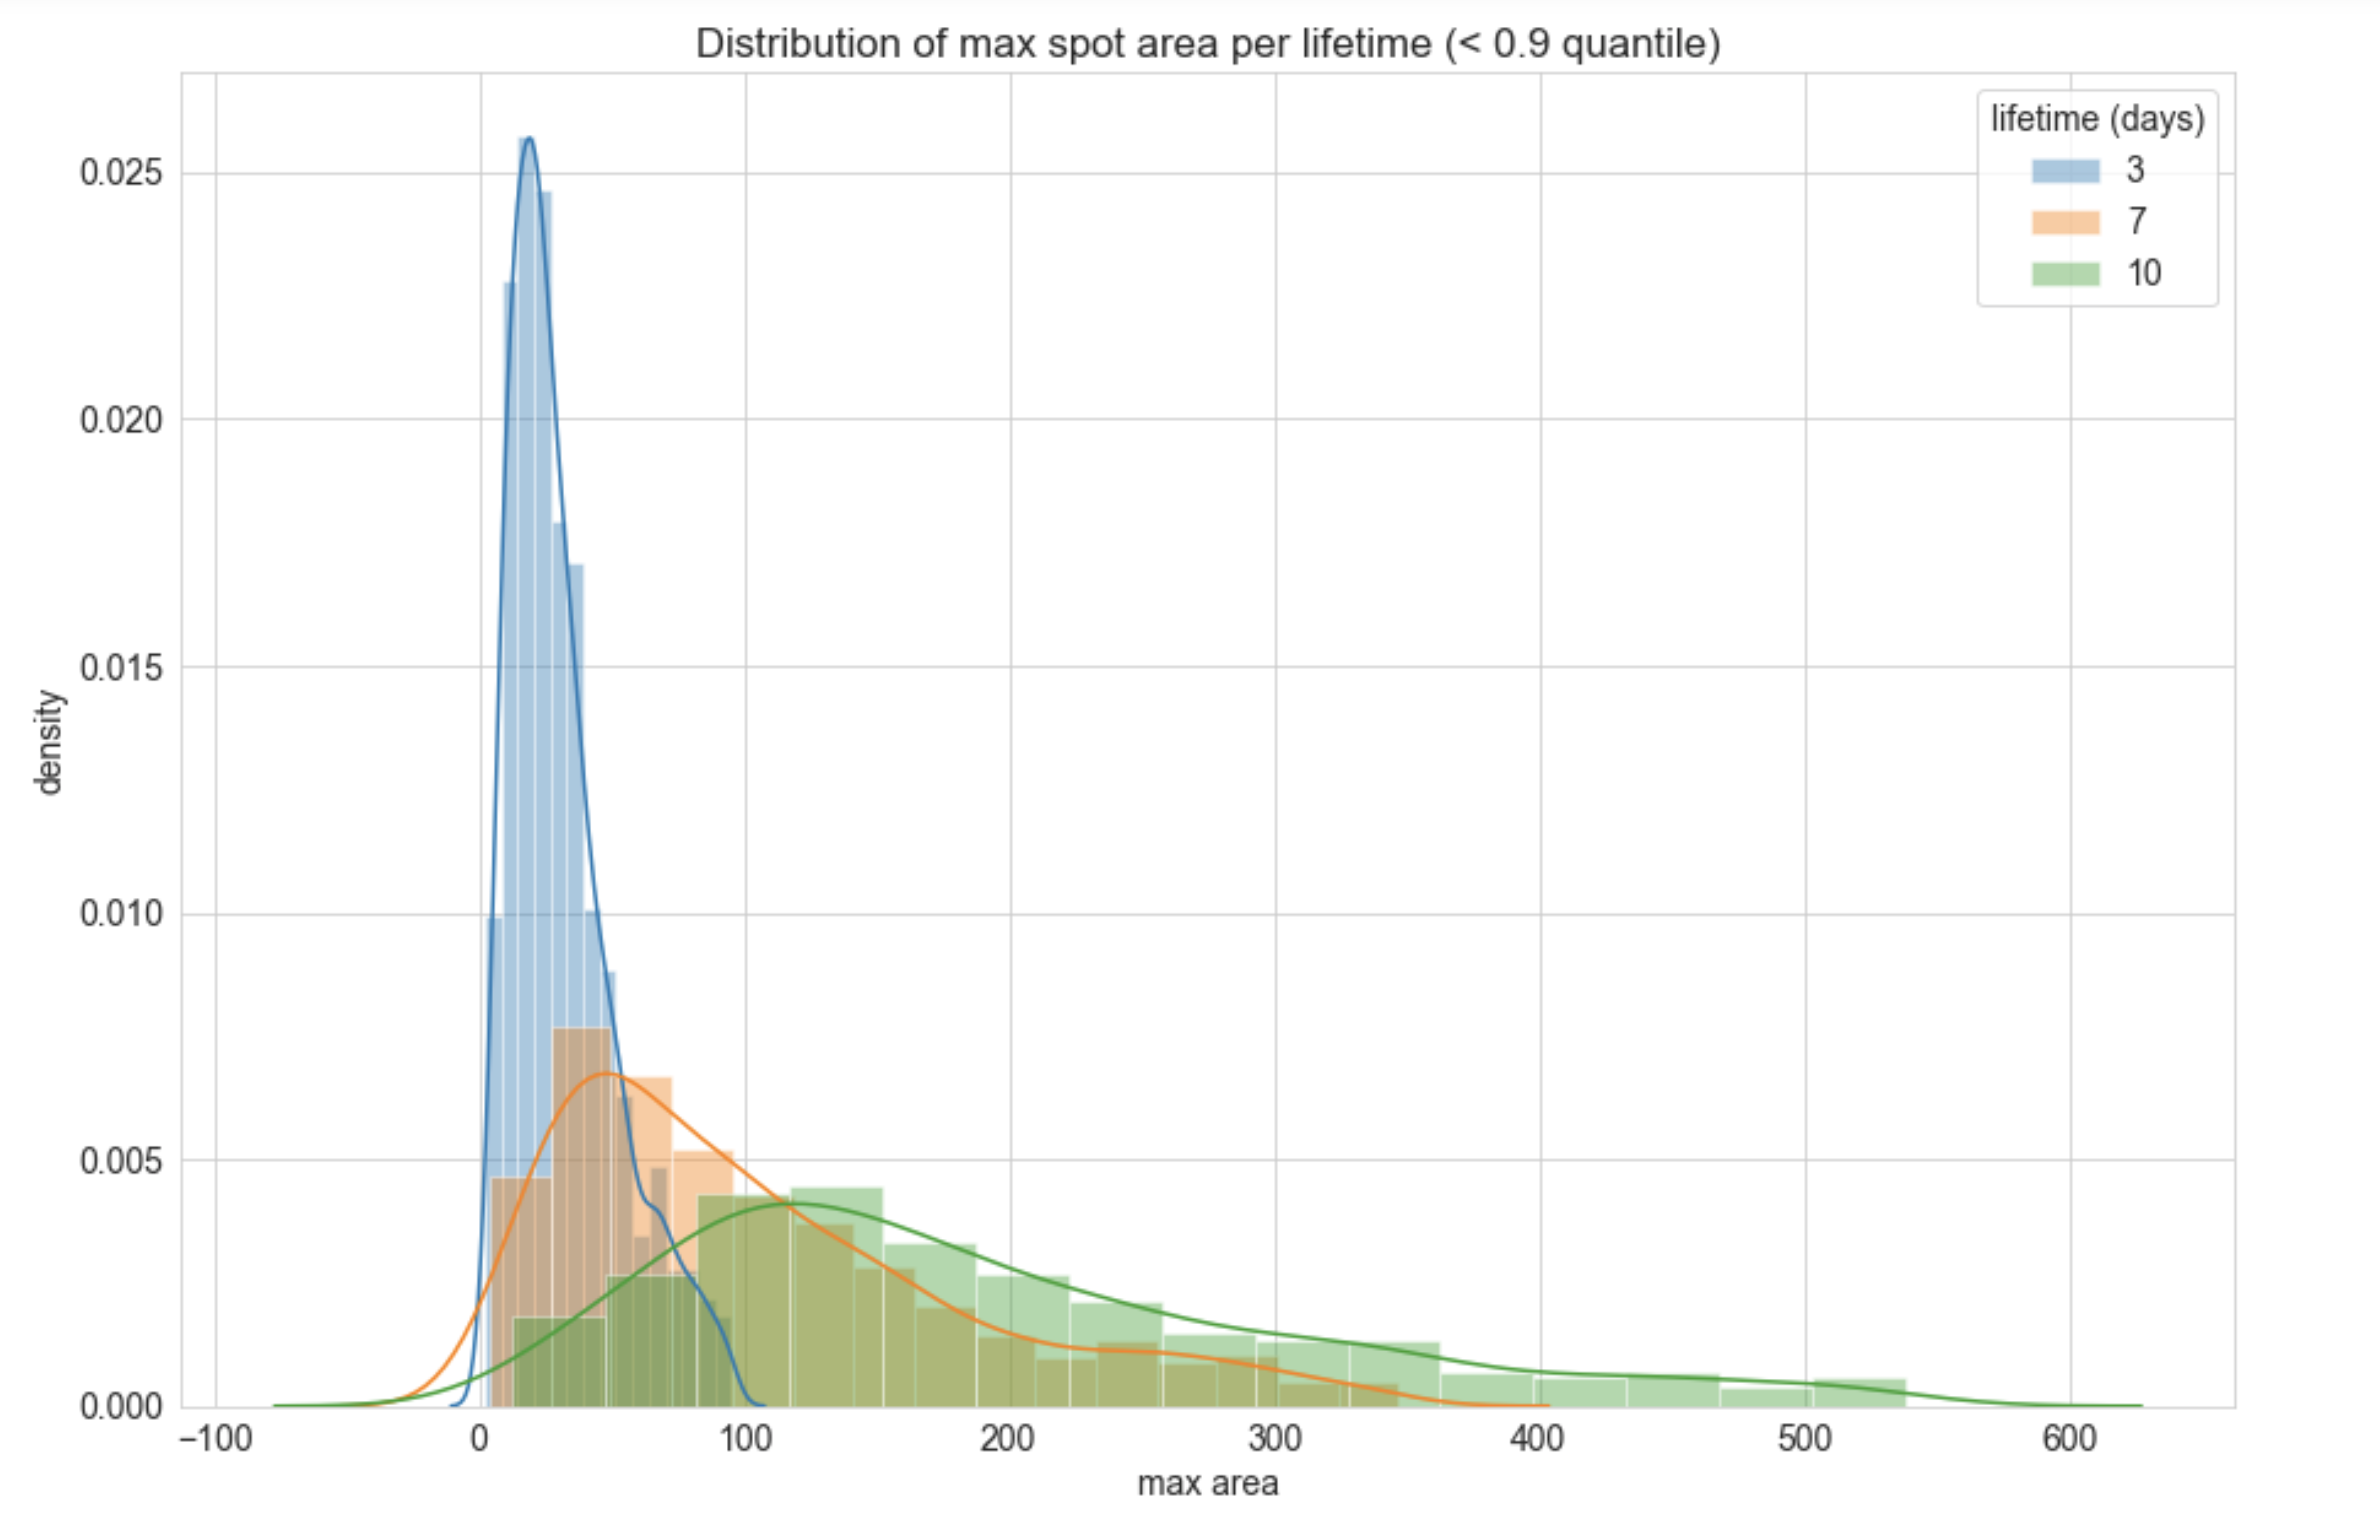
\includegraphics[width=17cm]{max_area_distr.png}
    \caption{Плотность распределения максимальной площади группы в зависимости от времени жизни группы.}
    \label{fig:my_label}
\end{figure}{}

На рис. 4.3 изображена плотность распределения максимальной площади группы для трех показателей времени жизни: 3, 7 и 10 дней (при этом у распределения отбрасывался ''хвост'', больший 0.9 квантиля). Легко видеть, что распределение смещается в сторону больших площадей с ростом времени жизни пятен. Таким образом, долгоживущие солнечные пятна, которые являются основным объектом исследования, в основном имеют площадь порядка нескольких сотен $\mu$Hem.

Помимо прочего, данные содержат пропуски, которые тоже приходится учитывать. Они также связаны с плохой видимостью солнечного диска. Характерный пример возникновения пропуска такой: какая-то группа пятен наблюдалась в течение нескольких дней, затем на 1-2 дня исчезла из наблюдения и снова появилась через несколько дней. При этом, такая серия наблюдений была помечена одним и тем же номером, а значит, создатели базы данных отнесли эти наблюдения к одной группе. Таких групп оказывается относительно немного (порядка 2500 при общем числе групп около 30000), поэтому их можно безболезненно исключить из рассмотрения.

Итак, фильтрация исходных данных включает в себя несколько составляющих (значения параметров принимаются такими же, как в \bibref{hathaway}{Hathaway D.H., Choudhary D.P.}{2008}):

\begin{enumerate}
    \item В итоговой выборке остаются только центральные фрагменты историй наблюдений: фиксируется некоторый порог $\varphi_\text{max}$, и в выборку включаются только те наблюдения, для которых долгота оказывается меньше по абсолютной величине, чем $\varphi_\text{max}$. Значение параметра было установлено в $\varphi_\text{max} = 60^\circ$.
    \item В выборку попадают только те наблюдения, что превосходят по площади некоторую минимальную $S_\text{min}$. Значение параметра принималось равным $S_\text{min} = 35 \, \mu\text{Hem}$.
    \item Из выборки исключаются все группы пятен, в истории наблюдений которых есть пропуски.
\end{enumerate}

\begin{figure}[H]
    \centering
    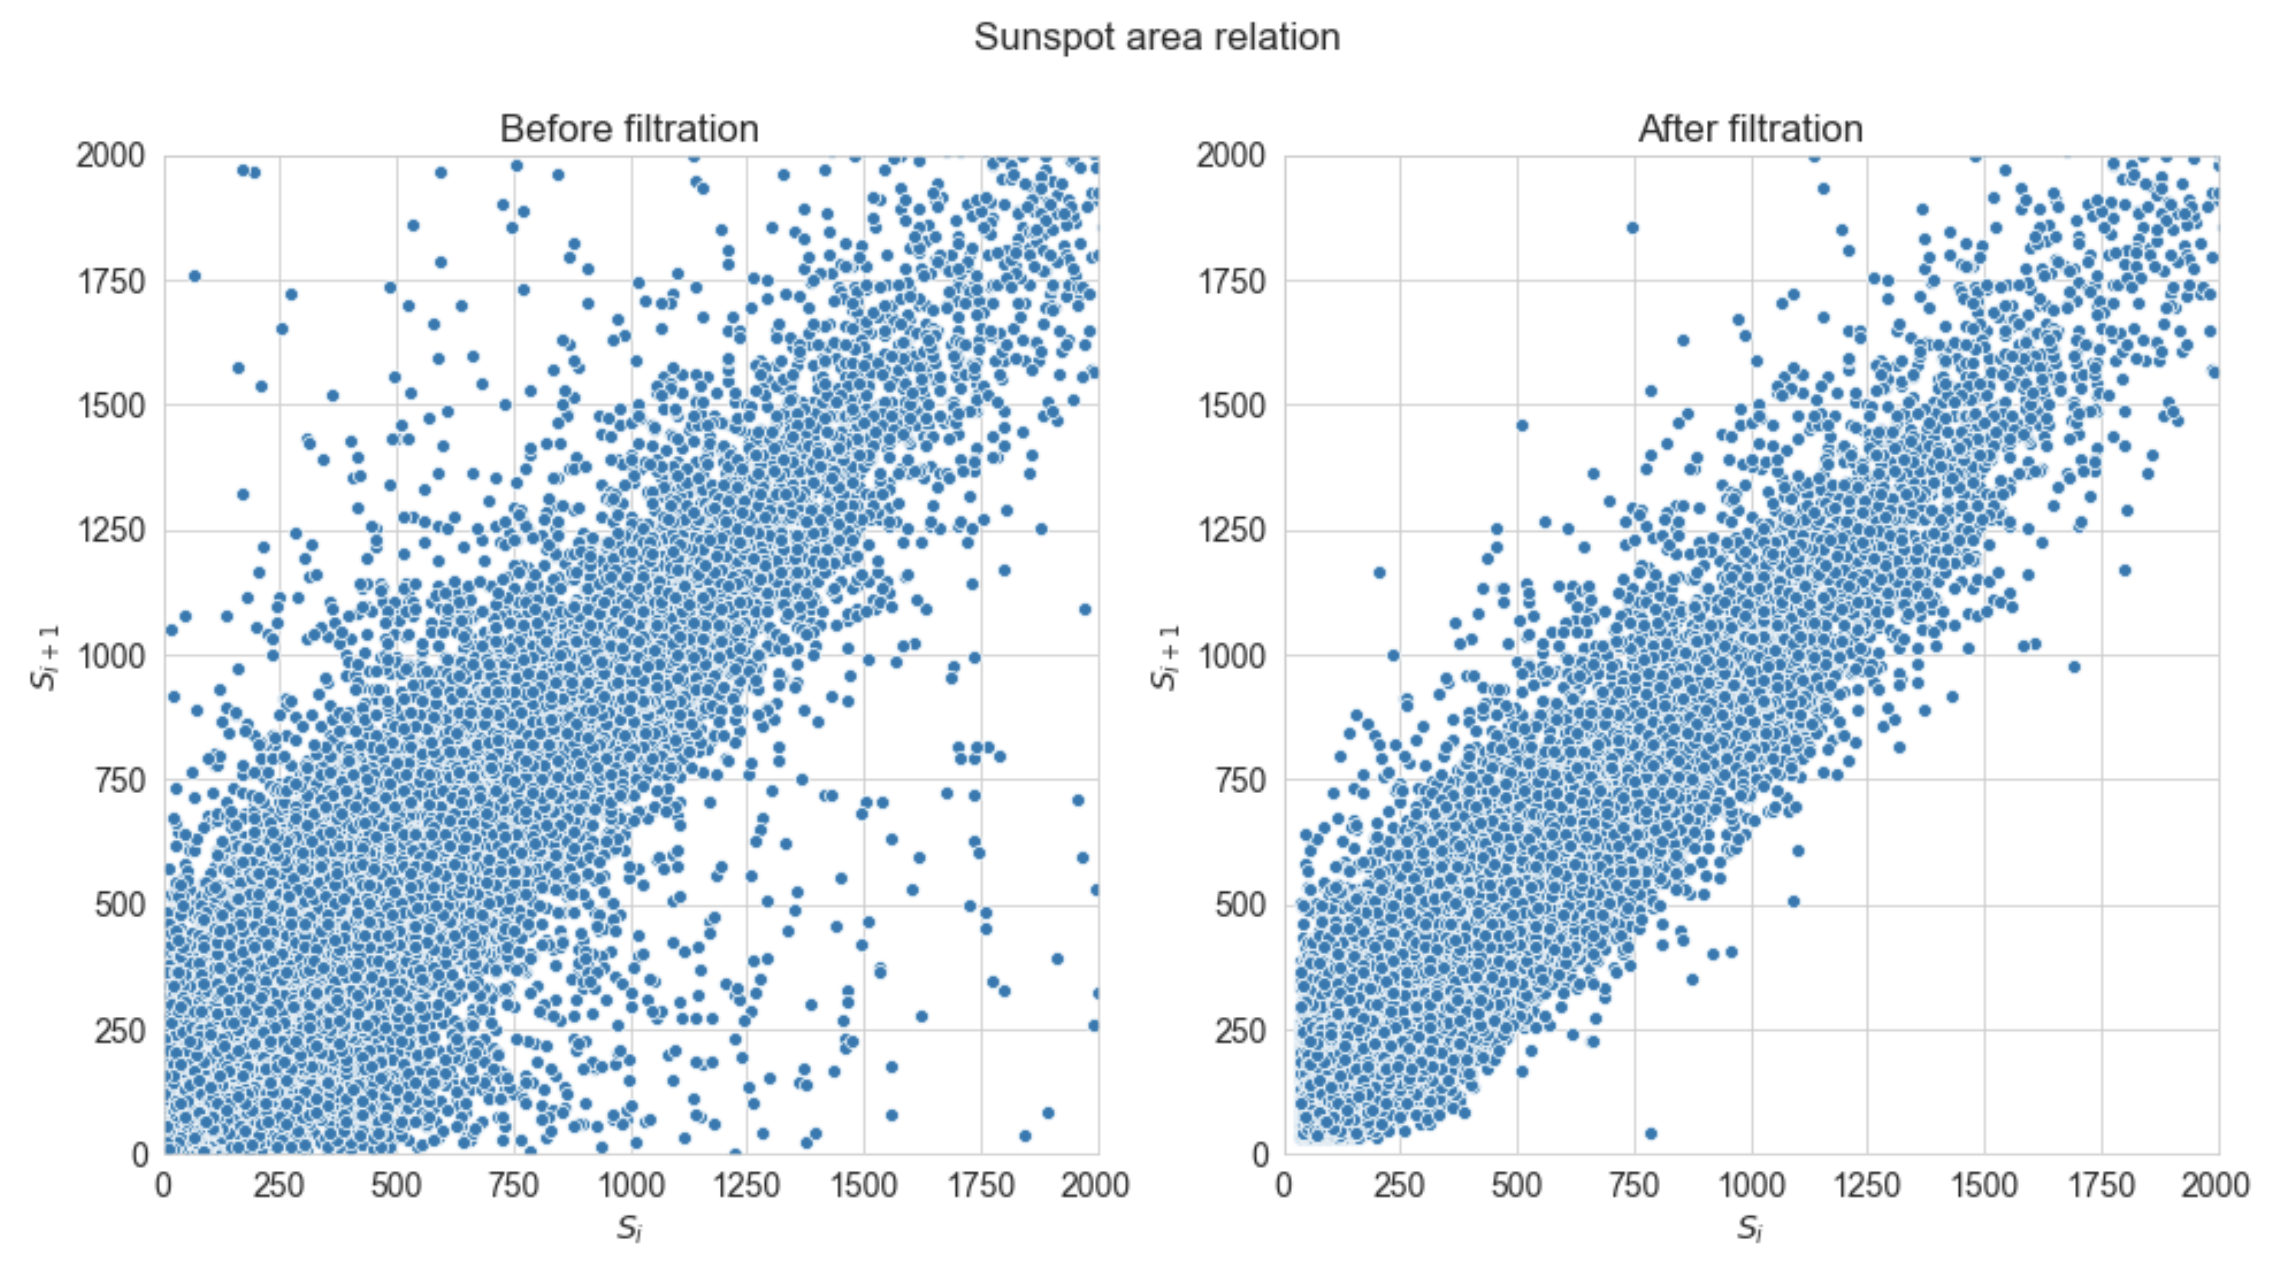
\includegraphics[width=17cm]{area_relation.png}
    \caption{Соотношение наблюдаемых площадей групп пятен до (слева) и после (справа) фильтрации.}
    \label{fig:my_label}
\end{figure}{}

Результаты такой фильтрации продемонстрированы на рис. 4.4. Обозначим за $S_i$ площадь некоторой группы пятен на $i$-ый день наблюдения, соответственно, $S_{i+1}$ - это площадь группы на следующий, $i+1$-ый день. Каждая точка на рис. 4.4 обозначает пару $(S_i, S_{i+1})$, причем левый график соответствует исходной базе данных, а правый - после применения описанного выше метода фильтрации. Этот рисунок демонстрирует, во-первых, сильную зашумленность исходных данных, а во-вторых, эффективность предложенного метода фильтрации (уменьшается разброс площадей, становится более четким линейный характер зависимости).

Обобщая все вышесказанное, исходные данные оказываются несовершенными и сильно зашумленными, что может оказать негативный эффект при обучении регрессионных моделей, однако использованный метод фильтрации относительно успешно с этим справляется, снижая шумовую компоненту в данных.

\section{Базовые модели}

\subsection{Векторная трансформация}

В рамках этой работы рассматривались модели, принимающие в качестве признакового описания векторы площади фиксированной длины, которую в дальнейшем будем обозначать за $d$. В результате фильтрации база данных превратилась в набор последовательностей из наблюдений за группами пятен. Для формирования обучающей и тестовой выборки необходимо сформировать из таких последовательностей векторы площадей и целевые значения площади.

Допустим, после фильтрации образовалась последовательность наблюдений площади $(S_1, S_2, ..., S_n)$. Можно покрывать эту последовательность ''окном'' длины $d+1$, тогда первые $d$ значений будут представлять некоторое признаковое описание наблюдений, а $d+1$-ое значение будет целевым. Получится не что иное, как предсказание следующего элемента последовательности по $d$ предыдущим. Такая трансформация записана в уравнении 5.1, в котором признаковые описания обозначены за $x_i$, а целевые значения площади - за $y_i$.

\begin{gather}
\begin{pmatrix}
    S_1 \\
    S_2 \\
    \vdots \\
    S_n
\end{pmatrix} \rightarrow
\Big\{(x_i, y_i) \Big| i = 1, ..., n - d \Big\}, \text{где }
x_i = \begin{pmatrix}
    S_i \\
    S_{i + 1} \\
    \vdots \\
    S_{i + d - 1} \\
\end{pmatrix}, y_i = S_{i + d}
\end{gather}

В дальнейшем все отфильтрованные последовательности разделялись на обучающие и тестовые, после чего к первым применялась описанная выше векторная трансформация, и получившиеся пары $(x_i, y_i)$ применялись для обучения регрессионных моделей.

\subsection{Метрики}

Обозначим за $\{(x_i, y_i)\}_{i=1}^l$ всю выборку, полученную в результате векторной трансформации, а за $a(x_i)$ предсказание модели на векторе $x_i$. Первоначально в ходе исследования было решено использовать ошибку MSE (Mean Squared Error, уравнение 5.2) как количественный показатель для измерения качества моделей.

\begin{equation}
    \text{MSE}(a, X, y) = \frac{1}{l} \sum_{i=1}^l \Big(y_i - a(x_i)\Big)^2
\end{equation}

Однако, у такого подхода к оцениванию модели есть значительный недостаток. Рассмотрим следующий простой пример. Пусть для двух объектов целевые значения площади равны $y_1 = 50$ и $y_2 = 500$, при этом предсказания модели на этих объектах равны, соответственно, $a(x_1) = 100$ и $a(x_2) = 550$. С точки зрения качества регрессии, предсказание алгоритма для второго объекта нужно признать куда более удачным, однако вклад в ошибку эти два предсказания вносят одинаковый: $(50 - 100)^2  = 50^2 = (500 - 550)^2$. Таким образом, модели важнее правильно попадать в порядок площади, чем в ее точное численное значение. По этой причине логичным представляется использовать ошибку MSLE (Mean Squared Logarithmic Error, уравнение 5.3). Эта метрика и применялась как основная для оценки количественных показателей модели. Ее применение здесь допустимо, поскольку все целевые значения площади неотрицательны (более того, в результате фильтрации они оказались больше порогового значения $S_\text{min} > 0$).

\begin{equation}
    \text{MSLE}(a, X, y) = \frac{1}{l} \sum_{i = 1}^l \Big(\log{y_i} - \log{a(x_i)} \Big)^2
\end{equation}

\subsection{Регрессионные модели}

В качестве базовых алгоритмов для регрессии применялись максимально простые модели по причине, во-первых, невысокой размерности признакового пространства, а во-вторых, сильной зашумленности данных (более сложные модели могут настроиться на шум и извлечь из данных несуществующие закономерности). В ходе этой работы были рассмотрены три модели, подробно они будут описаны в этом разделе. Примем такие обозначения для вектора площадей и целевого значения площади: $x = (S_1, ..., S_d), y = S_{d+1}$ \\

$\bullet$ \textbf{Линейная регрессия}

Предсказание алгоритма строится как линейная комбинация площадей с предыдущих наблюдений (уравнение 5.4), обучение весов $\alpha$ идет на минимизацию ошибки MSE.

\begin{equation}
    S_{d+1} \approx a(x) = \alpha_0 + \alpha_1 S_1 + ... + \alpha_d S_d
\end{equation}{}

Стоит отметить, что эта модель нужна только для сопоставления результатов, и ее не планируется использовать для анализа поведения солнечных пятен (например, по той причине, что эта модель не запрещает отрицательные предсказания, что противоречит физическому смыслу площади, а также работает в предположении линейной зависимости площади от предыдущих площадей). \\

$\bullet$ \textbf{Логарифмическая линейная регрессия}

Этот алгоритм также принадлежит к классу линейных моделей, однако он, в отличие от обычной линейной регрессии, призван оптимизировать ошибку MSLE напрямую. Для этого предсказывается не сама целевая площадь, а ее логарифм. Поскольку признаковое описание имеет такой же физический смысл, то и в качестве признаков для этой модели используются логарифмы площади. В итоге модель описывается уравнением 5.5.

\begin{equation}
    \log S_{d + 1} \approx \log a(x) = \alpha_0 + \alpha_1 \log S_1 + ... + \alpha_d \log S_d
\end{equation}

Экспоненциируя уравнение 5.5, получаем итоговую формулу для предсказания площади группы (уравнение 5.6). Модель обучается на минимизацию MSLE или, что эквивалентно, на минимизацию MSE для логарифма модели (уравнение 5.7). В программной реализации этой модели использовалась функция $\log(1 + x)$ вместо $\log(x)$, чтобы модель могла обрабатывать нулевые площади (таковые могут возникать, если для некоторой группы пятен в тестовой выборке не набирается $d$ наблюдений для формирования полного вектора, отчего первые несколько координат заполняются нулями). Однако, в большинстве своем площади групп $S \gg 1$, потому такое изменение незначительно влияет на модель.

\begin{equation}
    S_{d + 1} \approx a(x) = \exp \Big(\alpha_0 + \alpha_1 \log S_1 + ... + \log S_d \Big) = c_0 \, S_1^{\alpha_1} ... \, S_d^{\alpha_d}, \text{где } c_0 = e^{\alpha_0}
\end{equation}

\begin{equation}
    \argmin_\alpha \text{MSLE}(a, X, y) = \argmin_\alpha \text{MSE}(\log a, \log X, \log y)
\end{equation}

Использование этой модели является более осмысленным, чем стандартной линейной регрессии, поскольку она оптимизирует непосредственно ошибку RMSLE, а также всегда предсказывает положительные площади, что соответствует их физическому смыслу. \\

$\bullet$ \textbf{Метод $k$-ближайших соседей}

Поскольку признаковые описания представляются в виде векторов площадей, то разумным решением кажется попробовать метрические алгоритмы для регрессии. Метод $k$-ближайших соседей был выбран как самый простой представитель семейства метрических алгоритмов. К тому же, он хорошо интерпретируем: значение площади, приписываемое данной группе пятен, появляется из историй наблюдений, похожих на данную. В качестве функции расстояния в работе использовалась стандартная евклидова метрика.

\subsection{Оценивание моделей}

Существует два способа оценивания качества регрессионных моделей. Первый, более простой из них, заключается в проведении векторной трансформации для тестовых последовательностей и измерении ошибки на получившихся парах $(x, y)$ (по формулам 5.2 и 5.3). Другой подход основан на долгосрочном прогнозе площадей групп пятен. Поскольку ставится задача предсказания элементов последовательности, то разумно требовать от алгоритма не только точности однодневного прогноза, но и соответствия поведению группы пятен на протяжении нескольких дней. Осуществить такое оценивание можно, применяя обученные модели последовательно, стартовав с некоторого начального вектора площадей размерности $d$. Разберем подробнее, как будет строится предсказание для последовательности.

Обозначим тестовую выборку за $\mathcal{S}$. Пусть она содержит последовательность $(S^i_1, ..., S^i_{n_i})$ (здесь $i = 1, ..., l$ - верхний индекс, обозначает номер последовательности в выборке). Будем строить по ней новую последовательность $(\widehat{S}^i_1, ..., \widehat{S}^i_{n_i})$ с помощью предсказаний алгоритма. Первые $d$ элементов новой последовательности будут совпадать с элементами исходной последовательности (своеобразная ''база'' для регрессии): $\widehat{S}^i_j = S^i_j, j = 1, ..., d$. Остальная последовательность будет строится по предыдущим: $\widehat{S}^i_j = a\big((\widehat{S}^i_{j-d}, ..., \widehat{S}^i_{j-1})\big), j = d + 1, ..., n_i$, где $a$ - оцениваемая модель, и ошибка будет считаться только по таким элементам последовательности (всего их $n_i - d$). Обозначим за $N = \sum_{i=1}^l (n_i - d)$ - общее число прогнозов по всем последовательностям тестовой выборки. Тогда ошибки MSE и MSLE для долгосрочного прогноза определяются уравнениями 5.8 и 5.9.

\begin{equation}
    \text{MSE}(a, \mathcal{S}) = \frac{1}{N} \sum_{i=1}^l \sum_{j=d+1}^{n_i} (S^i_j - \widehat{S}^i_j)^2
\end{equation}

\begin{equation}
    \text{MSLE}(a, \mathcal{S}) = \frac{1}{N} \sum_{i=1}^l \sum_{j=d+1}^{n_i} (\log S^i_j - \log \widehat{S}^i_j)^2
\end{equation}

Таким образом, для всех моделей оценивалось качество как однодневного, так и многодневного прогноза. Впрочем, для лучшей интерпретируемости ошибок применялись RMSE (Root Mean Squared Error) и RMSLE (Root Mean Squared Logarithmic Error), которые высчитываются по формулам 5.10 и 5.11.

\begin{equation}
    \text{RMSE}(a, X, y) = \sqrt{\text{MSE}(a, X, y)}
\end{equation}

\begin{equation}
    \text{RMSLE}(a, X, y) = \sqrt{\text{MSLE}(a, X, y)}
\end{equation}

\subsection{Подбор гиперпараметров}

Во всех упомянутых моделях размерность векторов $d$ рассматривается как гиперпараметр, кроме того метод $k$-ближайших соседей содержит гиперпараметр $k$ - число соседей. Эксперименты по оцениванию моделей проводились как для ошибки RMSE, так и для ошибки RMSLE.

\begin{figure}[H]
    \centering
    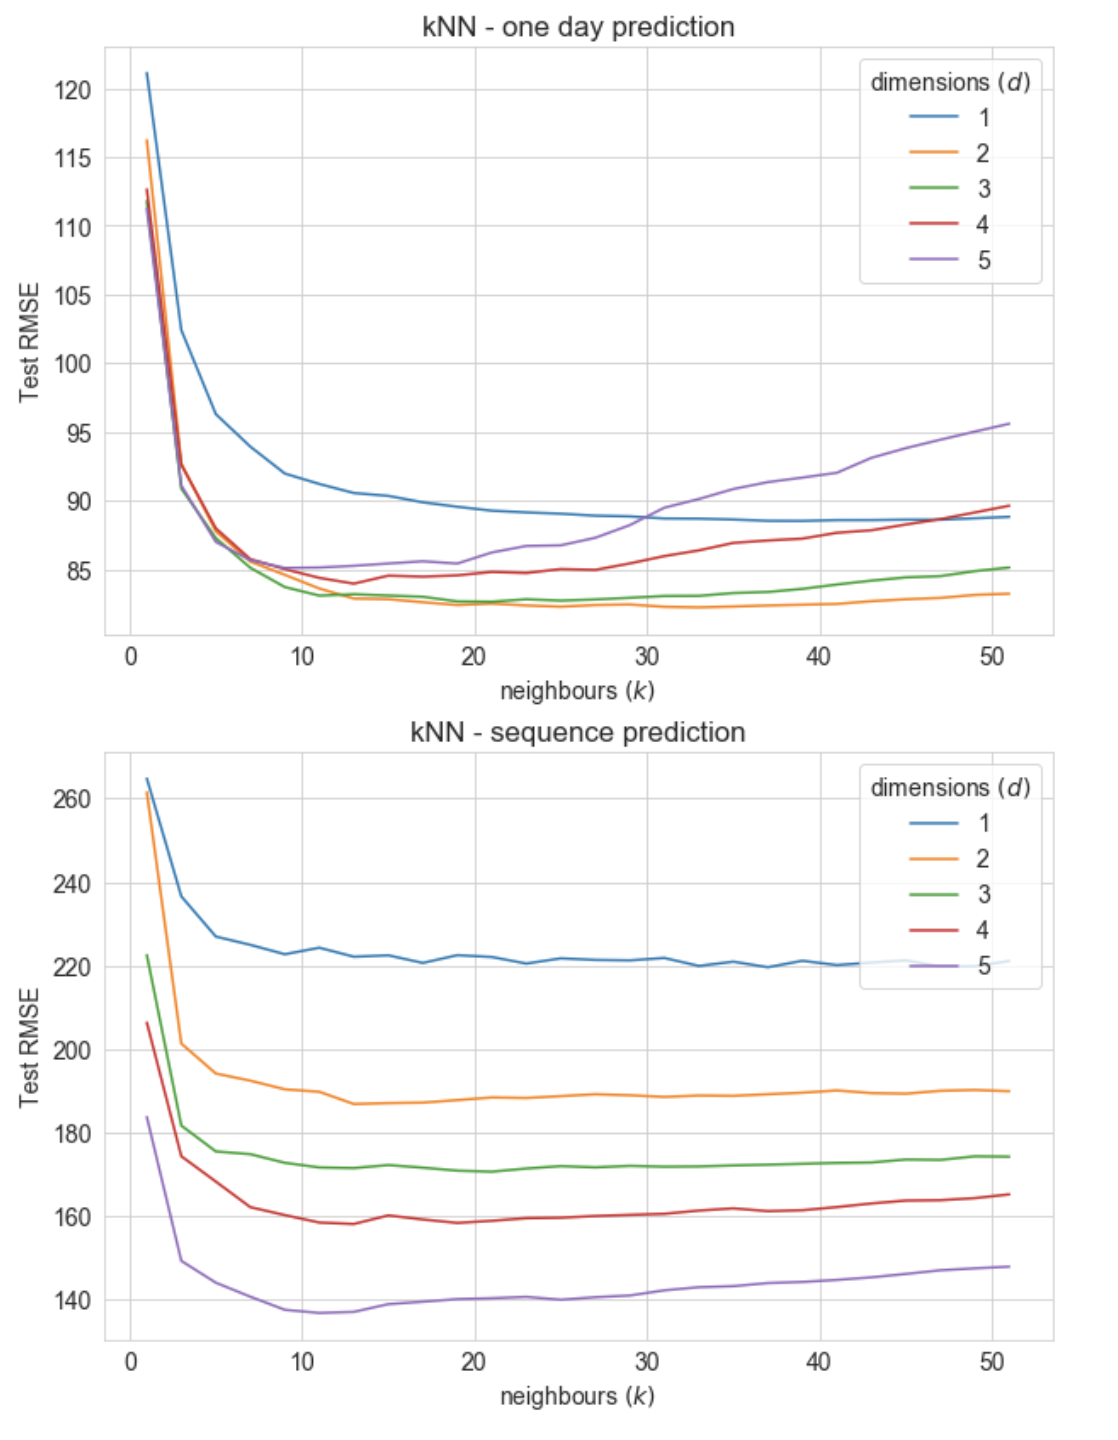
\includegraphics[width=11cm]{knn_rmse.png}
    \caption{Ошибка RMSE на тестовой выборке метода ближайших соседей при однодневном (сверху) и многодневном (снизу) прогнозе. По горизонтальной оси отложено число соседей $k$, разные кривые соответствуют разным размерностям векторов $d$.}
    \label{fig:my_label}
\end{figure}

На рис. 5.1 изображен подбор гиперпараметра $k$ для метода ближайших соседей. С точки зрения однодневного прогноза, наилучшими значениями гиперапараметров являются $d=2, 3$ и $k = 12, ..., 15$, при этом качество многодневного прогноза растет с увеличением размерности $d$, а наилучшее значения параметра числа соседей находится в окрестности значения $k=10$. Неожиданным результатом этого эксперимента является тот факт, что однодневный и многодневный прогноз в некотором смысле противоречат друг другу: оптимальные значения гиперпараметра $d$ у них принципиально разные. Неформально это можно объяснить так: увеличение размерности векторов приводит к увеличению точности многодневного прогноза, поскольку модель получает ''больше информации'' о последовательности (например, является ли последовательность возрастающей или убывающей и насколько быстро последовательность убывает).

\begin{figure}[H]
    \centering
    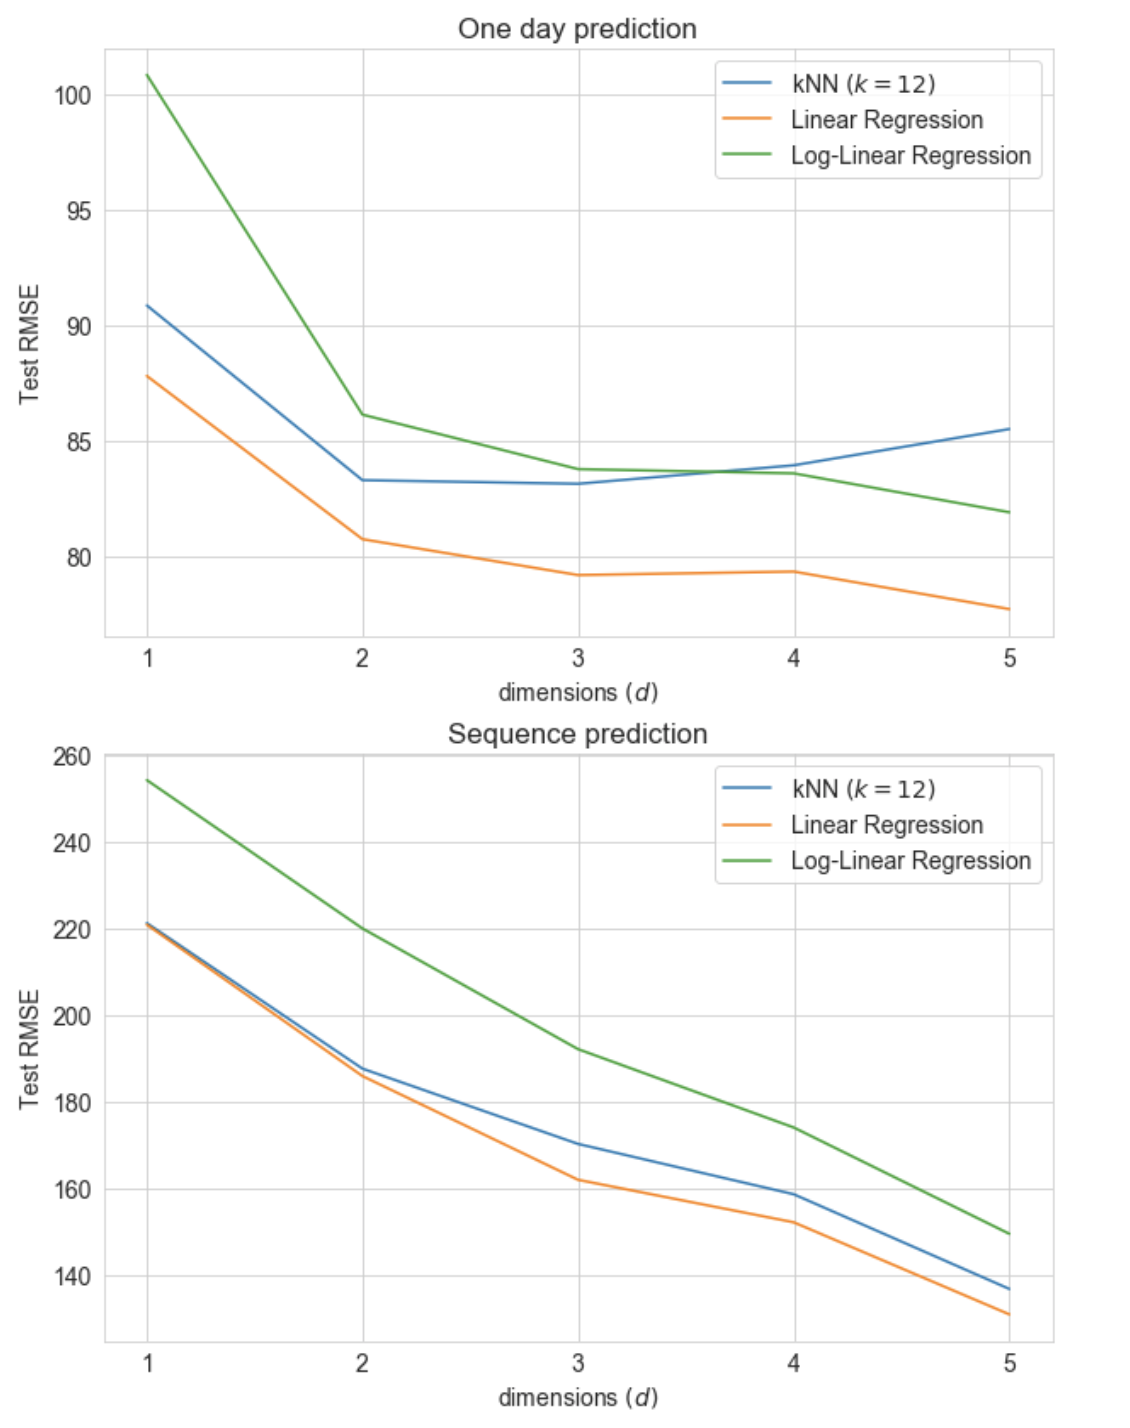
\includegraphics[width=11cm]{models_rmse.png}
    \caption{Ошибка RMSE на тестовой выборке разных моделей при однодневном (сверху) и многодневном (снизу) прогнозе. По горизонтальной оси отложена размерность векторов $d$, разные кривые соответствуют разным моделям.}
    \label{fig:my_label}
\end{figure}

На рис. 5.2 модели сравниваются по показателю ошибки RMSE на тестовой выборке для разных размерностей $d$. Для метода ближайших соседей число соседей было установлено одинаковым для всех размерностей и равным $k=12$. С точки зрения ошибки RMSE наилучшей моделью является линейная регрессия, что странно считать адекватным с учетом упомянутых недостатков линейной модели. По этой причине, более правильным количественным показателем стоит считать ошибку RMSLE.

\begin{figure}[H]
    \centering
    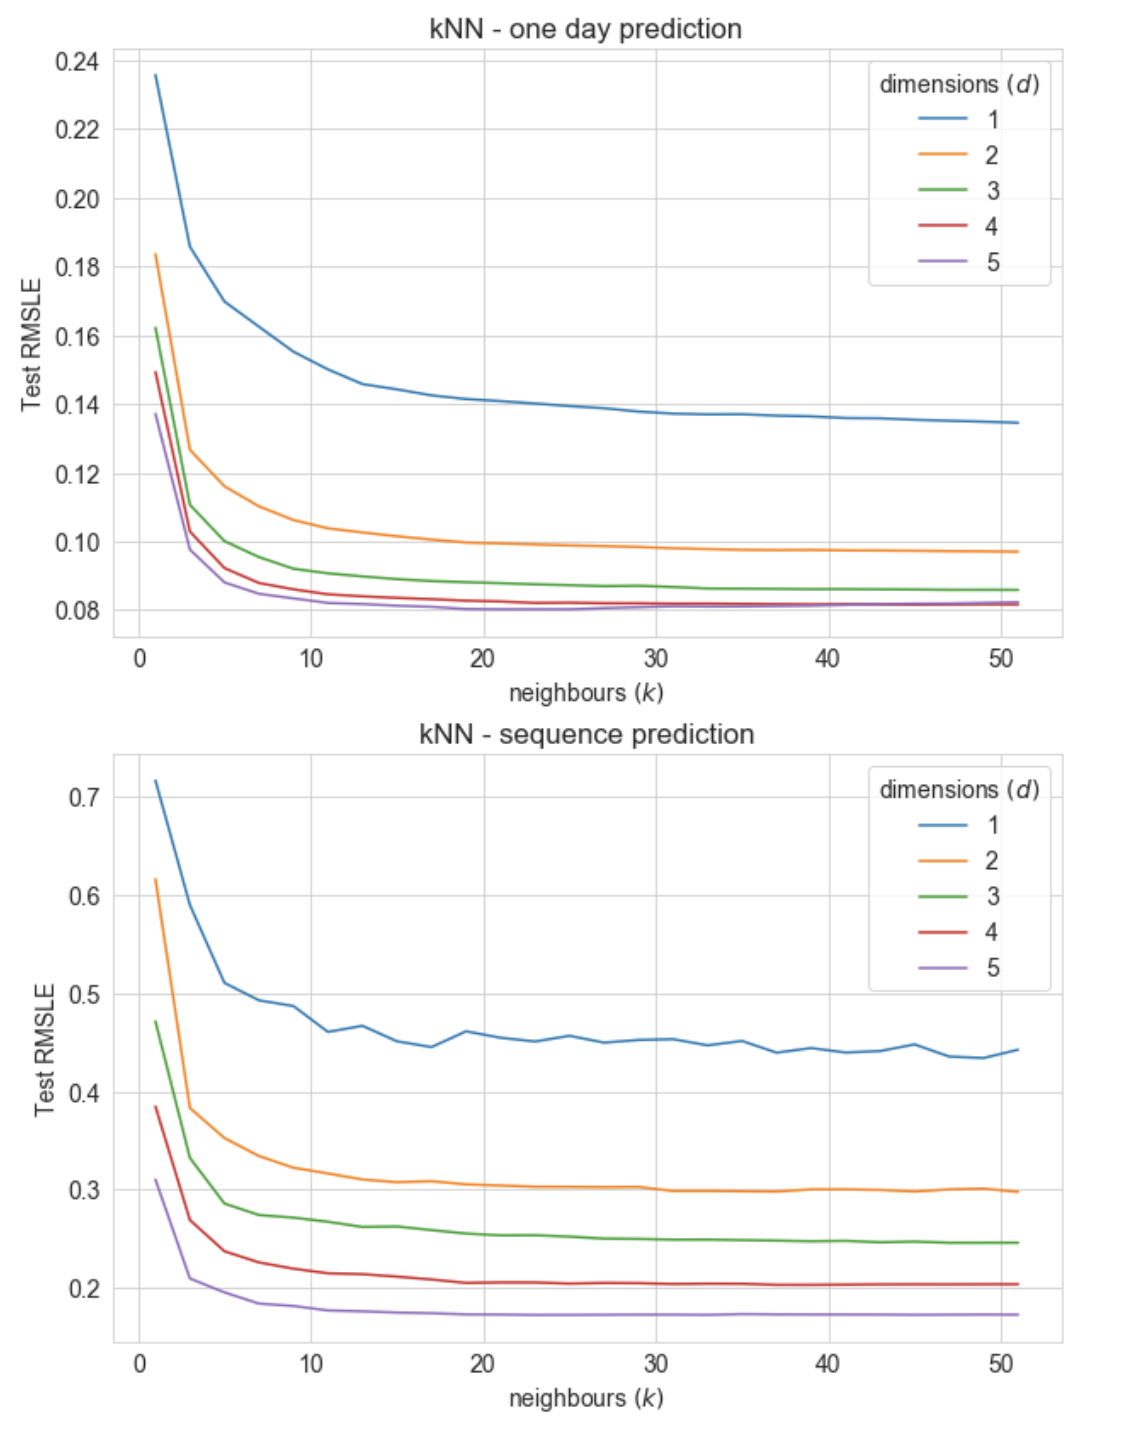
\includegraphics[width=11cm]{knn_rmsle.png}
    \caption{Ошибка RMSLE на тестовой выборке метода ближайших соседей при однодневном (сверху) и многодневном (снизу) прогнозе. По горизонтальной оси отложено число соседей $k$, разные кривые соответствуют разным размерностям векторов $d$.}
    \label{fig:my_label}
\end{figure}{}

Графики на рис. 5.3 демонстрируют ошибку RMSLE на тестовой выборке метода ближайших соседей (по аналогии с рис. 5.1). Здесь качество однодневного и многодневного прогноза гораздо лучше соотносятся друг с другом, чем для RMSE: ошибка монотонно уменьшается с ростом размерности векторов. Кроме того, качество выходит на плато с ростом числа соседей $k$.

\begin{figure}[H]
    \centering
    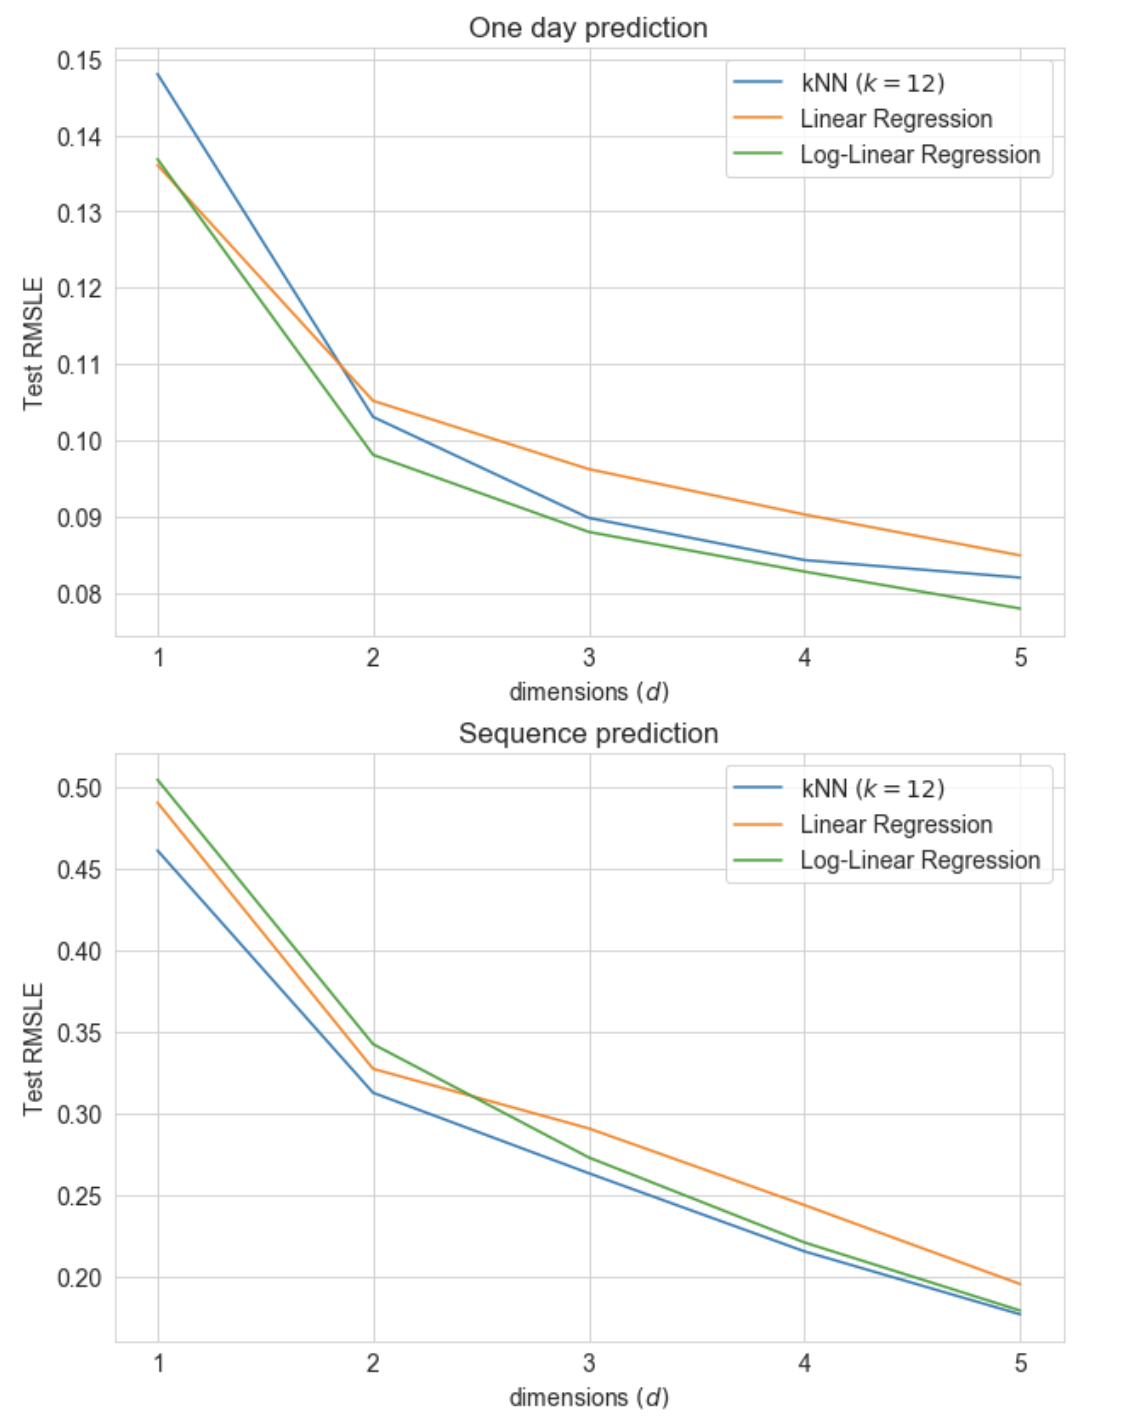
\includegraphics[width=11cm]{models_rmsle.png}
    \caption{Ошибка RMSLE на тестовой выборке разных моделей при однодневном (сверху) и многодневном (снизу) прогнозе. По горизонтальной оси отложена размерность векторов $d$, разные кривые соответствуют разным моделям.}
    \label{fig:my_label}
\end{figure}

Рис 5.4 перекликается с рис. 5.2, изображая качество моделей при варьировании размерности векторов $d$. Стоит отметить, что линейная регрессия может предсказывать отрицательную площадь, поэтому для валидного вычисления логарифмов ее прогноз должен быть скорректирован. Здесь применялась коррекция, описанная уравнением 5.12 ($a(x)$ обозначает исходное предсказание линейной регрессии, а $\widetilde{a}(x)$ - скорректированное).

\begin{equation}
    \widetilde{a}(x) = \max\{1, a(x)\}
\end{equation}

Логарифмическая линейная регрессия оказывается оптимальной с точки зрения однодневного прогноза (по той причине, что настраивается непосредственно на ошибку MSLE), но уступает в качестве методу ближайших соседей при переходе к многодневному прогнозу. При этом, ошибка всех моделей падает при увеличении размерности векторов $d$.

Из проведенной серии экспериментов следуют два ключевых вывода:

\begin{enumerate}
    \item Метод ближайших соседей оказался наилучшим с точки зрения ошибки RMSLE: он незначительно уступил логарифмической линейной регрессии при однодневном прогнозе, но превзошел ее при многодневном прогнозе. Поэтому именно метод ближайших соседей был выбран в качестве базовой модели для дальнейшего анализа.
    \item Качество моделей растет при увеличении размерности векторов $d$. Однако, зачастую история наблюдений оказывается недостаточной по размеру для формирования больших векторов (размерности $d=4, 5$). Поэтому при решении реальных задач можно ''доращивать'' истории наблюдений до нужного размера с помощью последовательного применения моделей для низких размерностей ($d=1, 2, 3, 4$), после чего уже использовать модель для максимальной размерности ($d=5$). Такую модель будем в дальнейшем именовать ''многоразмерной''.
\end{enumerate}

\section{Скорость убывания площади}

\subsection{Аналитическая формула}

С помощью разработанной модели можно оценить скорость убывания площади групп пятен. Наблюдения имеют ежедневный характер, и скорость убывания $D_i$ в $i$-ый день наблюдений за группой описывается уравнением 6.1.

\begin{equation}
    D_i = \frac{S_{i-1} - S_{i+1}}{2}
\end{equation}

При рассмотрении убывающих последовательность площадей $D_i > 0$. В работе предлагается использовать модель для сбора статистики по скорости убывания. Для этого использовалась многоразмерная модель на основе метода ближайших соседей со значением параметра $k=15$. Для обучения использовались только убывающие векторы площади. Максимальная используемая размерность модели $d=4$ (поскольку убывающих последовательностей размерности $d=5$ оказалось значительно меньше по количеству).

Однако, приходится учитывать несовершенства данных, описанных в разделе 4.1. В связи с этим, сбор статистики осуществлялся следующим образом:

\begin{enumerate}
    \item Предсказания алгоритма использовались для продления истории наблюдений для групп пятен, исчезающих за восточным лимбом Солнца (по аналогии с многодневным прогнозом, описанном в разделе 5.4). Поэтому продлевались истории тех пятен, для которых самое восточное наблюдение имеет долготу, большую $\varphi_{\max} = 60^{\circ}$. Предсказания продолжались до достижения минимального порога площади $S_{\min} = 45$ $\mu$Hem.
    \item Из выборки исключались те группы пятен, для которых первое наблюдение имеет долготу, меньшую $\varphi_{\min} = -60^{\circ}$, чтобы отсечь группы, пришедшие с западного лимба Солнца.
    \item Из оставшихся последовательностей рассматривались только те, что строго убывают после максимума. В выборку попадали такие последовательности, начиная с их максимума. Далее, из числа строго убывающих последовательностей исключались те, что имеют длину меньше $T=10$ дней (поскольку интерес представляет изучение долгоживущих пятен).
\end{enumerate}

Обозначим за $\sigma = \frac{S}{S_0}$ - отношение текущей площади группы к ее максимальной площади. После отбора последовательностей собиралась статистика величин $D$ и $\sigma$. Далее рассматривалась двухпараметрическая модель (с параметрами $\alpha, \gamma$), приближающая скорость убывания $D$ (уравнение 6.2).

\begin{equation}
    D \approx \alpha \sigma^{\gamma}
\end{equation}

Параметры обучались градиентным спуском на минимизацию ошибки MSLE (здесь она применяется из таких же соображений, что и для оценки качества базовых моделей). Пусть $\{(D_i, \sigma_i)\}_{i=1}^l$ - это собранная статистика, тогда ошибка $\mathcal{L}(\alpha, \gamma)$ описывается уравнением 6.3, ее градиент по параметрам - уравнениями 6.4 и 6.5.

\begin{equation}
    \mathcal{L}(\alpha, \gamma) = \frac{1}{2l} \sum_{i=1}^l \Big(\log(D_i) - \log(\alpha \sigma_i^{\gamma})\Big)^2
\end{equation}

\begin{equation}
    \frac{\partial \mathcal{L}(\alpha, \gamma) }{\partial \alpha} = \frac{1}{\alpha l} \sum_{i=1}^l \Big(\log(\alpha \sigma_i^{\gamma}) - \log(D_i) \Big)
\end{equation}

\begin{equation}
    \frac{\partial \mathcal{L}(\alpha, \gamma) }{\partial \gamma} = \frac{1}{l} \sum_{i=1}^l \Big(\log(\alpha \sigma_i^{\gamma}) - \log(D_i) \Big) \log(\sigma_i)
\end{equation}

Получившиеся оптимальные значения $\alpha^*, \gamma^*$ записаны в таблицу 6.1. Результат регрессии изображен на рис. 6.1.

\begin{table}[H]
\centering

\begin{tabular}{|M{2.2cm}|M{2.2cm}|}
\hline
$\alpha^*$ & $\gamma^*$ \\
\hline
$85.979$ & $0.514$ \\
\hline
\end{tabular}

\caption{\label{tab:table-name} Оптимальные значения параметров.}
\end{table}

Таким образом, имеет место приблизительная пропорциональность $D \propto \sqrt{\sigma} = \sqrt{\frac{S}{S_0}}$. Если принять $S \propto r^2$, где $r$ - радиус солнечного пятна, то получается $D \propto \frac{r}{r_0}$, а это и есть результат, полученный \bibref{petrovay}{Petrovay K., Van Driel-Gesztelyi L.}{1997}. Получается, что разработанная модель подтверждает формулу, полученную в указанном исследовании.

\begin{figure}[H]
    \centering
    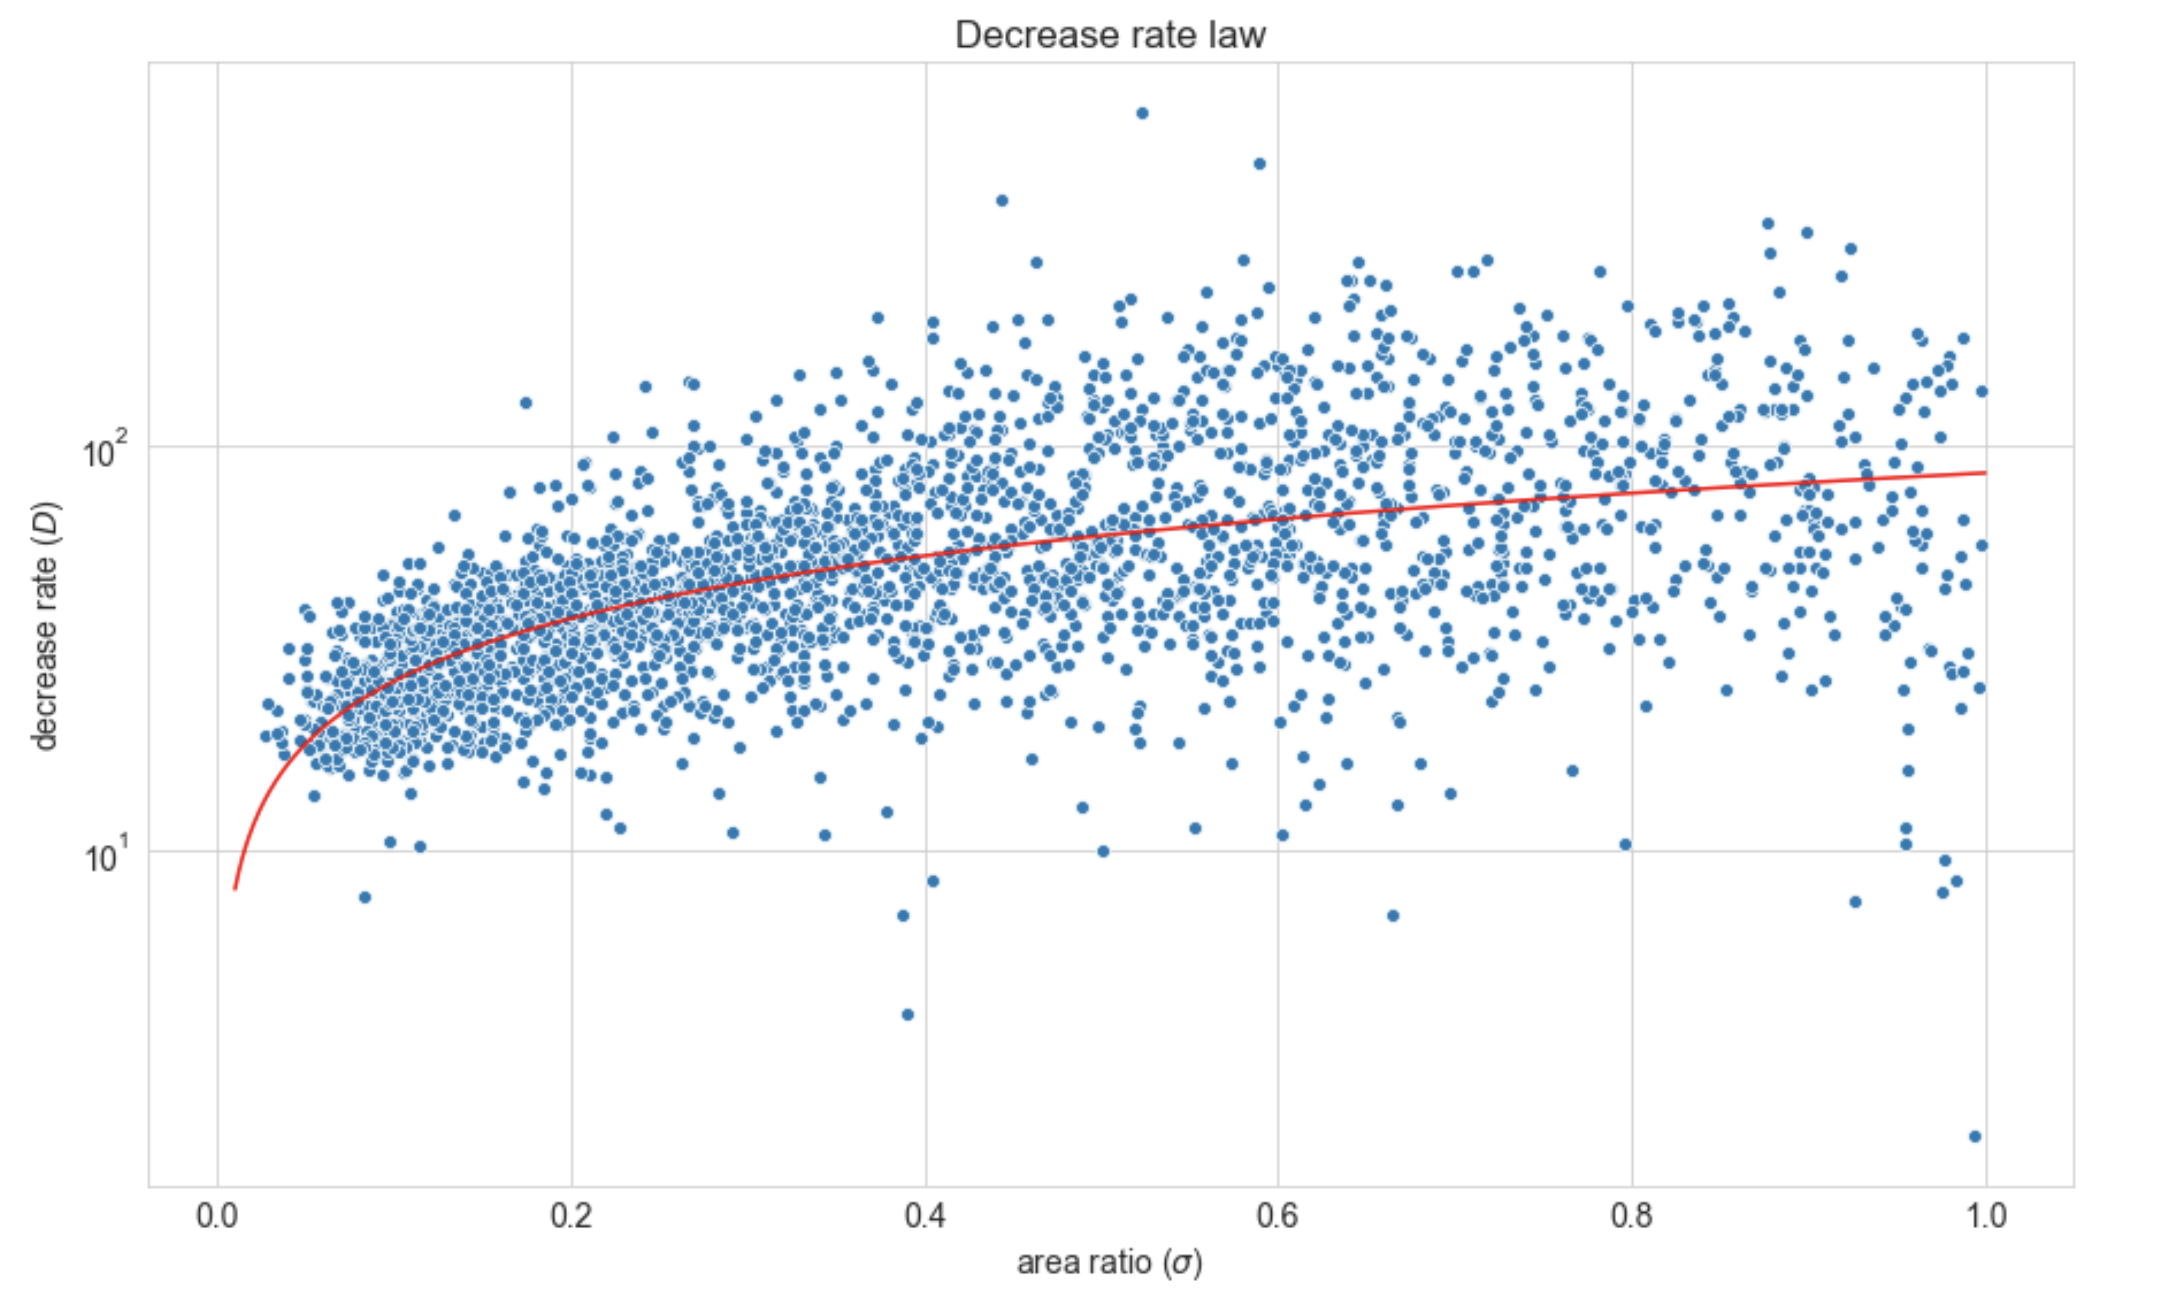
\includegraphics[width=17cm]{decrease_rate.png}
    \caption{Результат регрессии скорости убывания площади. Каждая точка на графике - пара $(\sigma_i, D_i)$, красная кривая задается уравнением $f(\sigma) = \alpha^* \sigma^{\gamma^*}$.}
    \label{fig:my_label}
\end{figure}

\subsection{Распределение}

Также было показано соответствие скорости убывания площади логнормальному распределению, что соотносится со статьей \bibref{hathaway}{Hathaway D.H., Choudhary D.P.}{2008}. В вычислительном пакете \bibref{scipy}{}{SciPy} плотность логнормального распределения задается параметрами $s, \theta$ и определяется уравнением 6.6.

\begin{equation}
    \rho(x) = \frac{1}{s\theta x \sqrt{2\pi}} \exp\left(-\frac{\log^2\left(x / \theta \right)}{2s^2}\right)
\end{equation}

Рассмотрим случайные величины $X \sim \mathcal{N}(\mu, \sigma^2), Y \sim \log \mathcal{N}(s, \theta)$ такие, что $X = \log(Y)$. Тогда их параметры связаны так: $s = \sigma, \theta = e^{\mu}$. Обозначим за $\widehat{\mu}$ и $\widehat{\sigma}$, соответственно, выборочное среднее и стандартное отклонение выборки $\log D$ (уравнения 6.7 и 6.8, предварительно у выборки отсекался ''хвост'', больший $0.975$ квантиля).

\begin{equation}
    \widehat{\mu} = \frac{1}{l}\sum_{i=1}^l \log(D_i)
\end{equation}

\begin{equation}
    \widehat{\sigma} = \sqrt{\frac{1}{l} \sum_{i=1}^l \big(\log(D_i) - \widehat{\mu}\big)^2}
\end{equation}

Обозначим $\widehat{s} = \widehat{\sigma}, \widehat{\theta} = e^{\widehat{\mu}}$ и рассмотрим распределение $\log \mathcal{N}(\widehat{s}, \widehat{\theta})$. Соответствие эмпирической плотности логнормальному распределению изображено на рис. 6.2. В целом, распределение скорости убывания плошади, которое получает алгоритм, хорошо описывается логнормальным.

\begin{figure}[H]
    \centering
    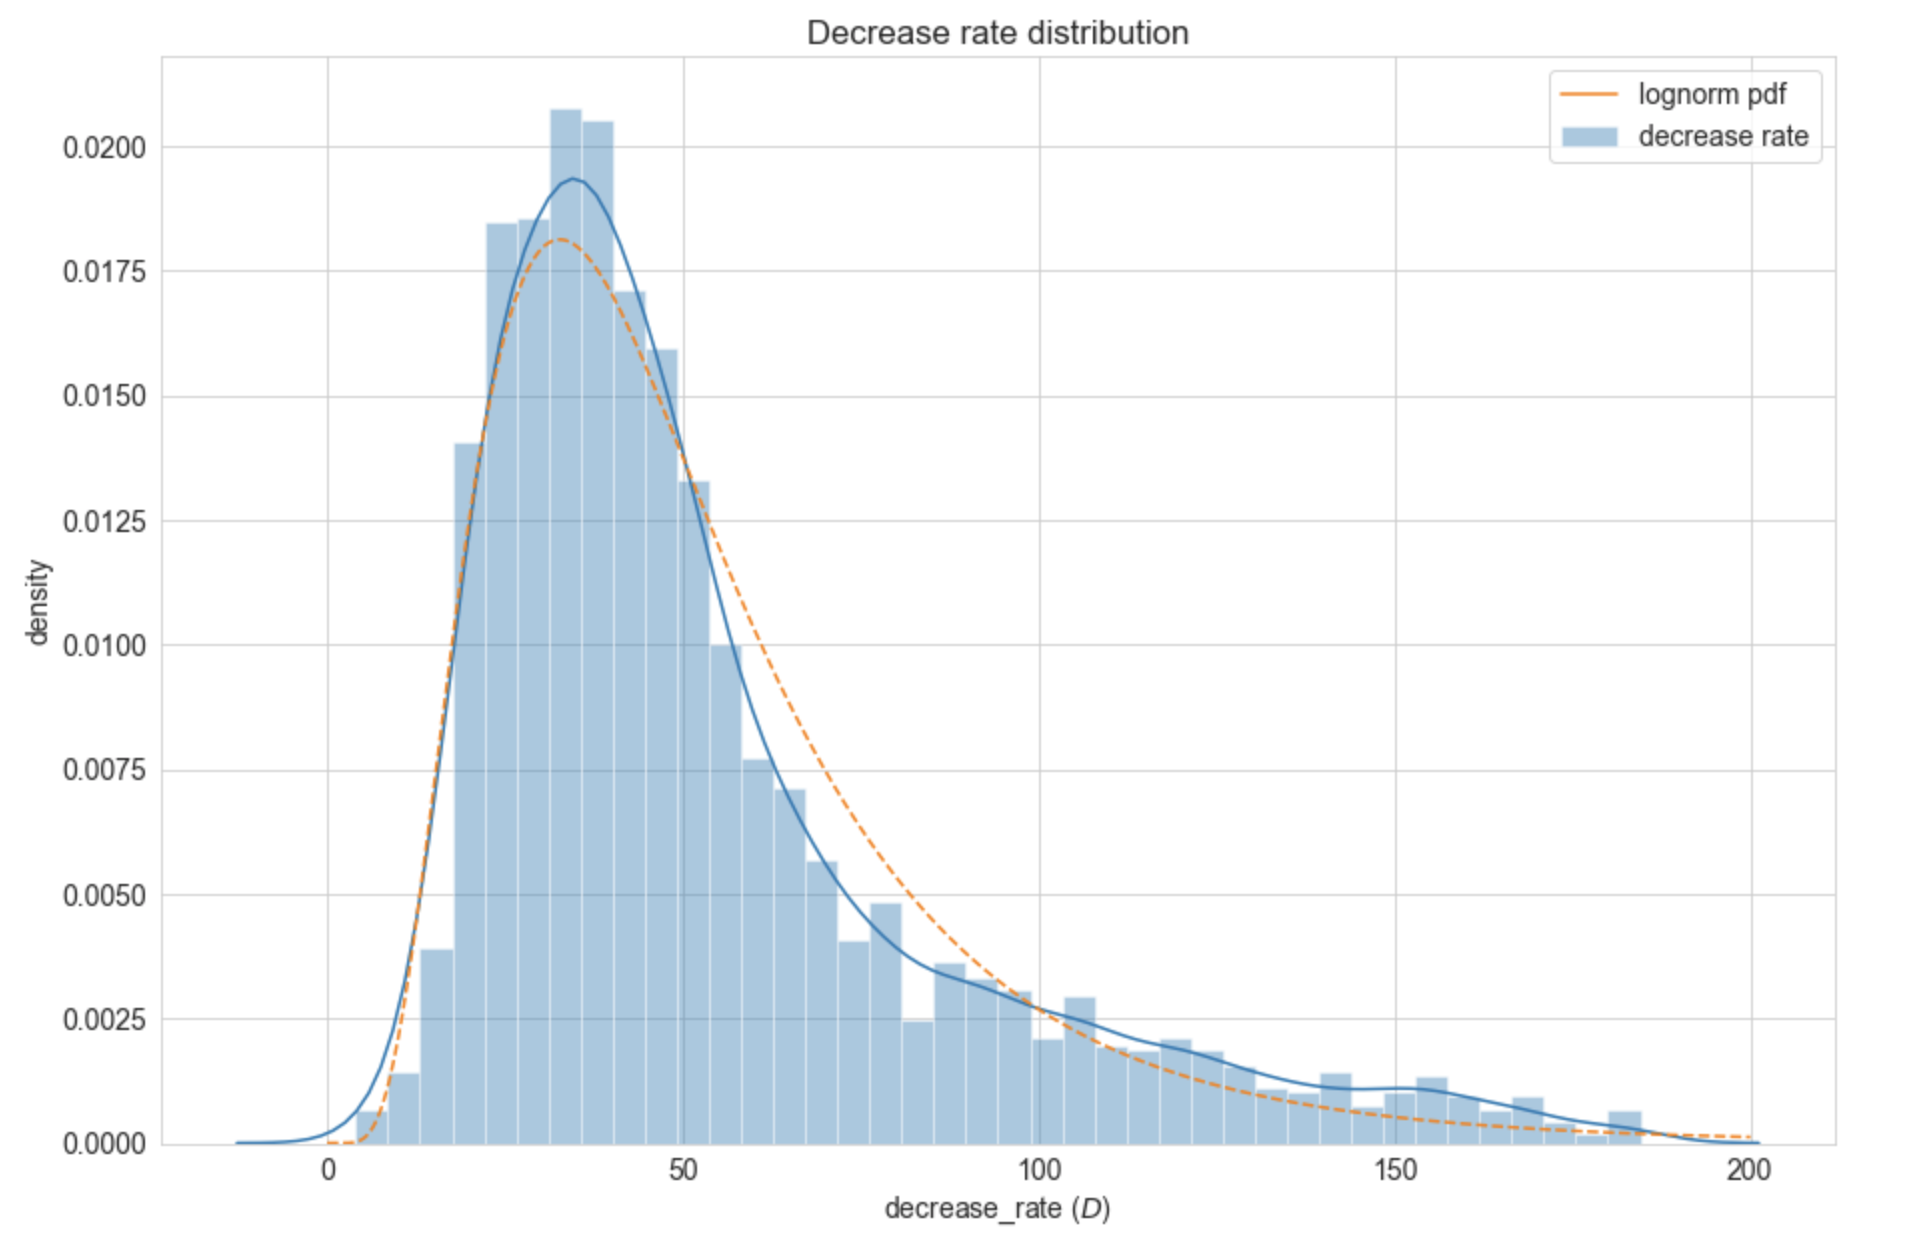
\includegraphics[width=17cm]{density.png}
    \caption{Плотность распределения скорости убывания площади. Синим цветом изображена эмпирическая плотность, оранжевым пунктиром - плотность $\log \mathcal{N}(\widehat{s}, \widehat{\theta})$.}
    \label{fig:my_label}
\end{figure}

\newpage
\section{Заключение}

В ходе этого исследования было рассмотрено несколько регрессионных моделей, из которых была отобрана наилучшая с точки зрения минимизации ошибки MSLE, таковой оказалась многоразмерная модель на основе метода ближайших соседей. Разработанный алгоритм использовался для вывода аналитической формулы для скорости убывания площади, полученный результат $D \propto \sqrt{\frac{S}{S_0}}$ совпал с \bibref{petrovay}{Petrovay K., Van Driel-Gesztelyi L.}{1997}. Также было продемонстрировано соответствие скорости убывания площади, получаемой алгоритмом, логнормальному распределению, что соотносится с одним из выводов в \bibref{hathaway}{Hathaway D.H., Choudhary D.P.}{2008}. Полученную модель можно применять в дальнейшем для решения других задач анализа солнечной активности (например, задачу получения правдоподобного распределения времени жизни солнечных пятен).

\newpage
\section{Список источников}

\begingroup
\renewcommand{\section}[2]{}
\begin{thebibliography}{}
\bibitem{bumba}\hypertarget{bumba}{}
\textit{Bumba V.} (1963) Development of spot group areas in dependence on the local magnetic field // Bulletin of the Astronomical Institute of Czechoslovakia, \textnumero\, 14, P. 91-96.

\bibitem{hathaway}\hypertarget{hathaway}{}
\textit{Hathaway D.H., Choudhary D.P.} (2008) Sunspot group decay // Solar Phys. (2008) \textnumero\, 250. P. 269-278.

\bibitem{petrovay}\hypertarget{petrovay}{}
\textit{Petrovay K., Van Driel-Gesztelyi L.} (1997) Making sense of sunspot decay // Solar Phys. (1997) \textnumero\, 166. P. 249-266.

\bibitem{rgo}\hypertarget{rgo}{}
\textit{Royal Observatory, Greenwich} USAF/NOAA Sunspot Data [Электронный ресурс] / Dr. David Hathaway. URL: \url{https://solarscience.msfc.nasa.gov/greenwch.shtml}, свободный. (дата обращения: 31.01.20).

\bibitem{scipy}\hypertarget{scipy}{}
\textit{SciPy} Lognormal distribution [Электронный ресурс] / The SciPy community. URL: \url{https://docs.scipy.org/doc/scipy/reference/generated/scipy.stats.lognorm.html}, свододный. (дата обращения: 14.05.20).
\end{thebibliography}{}
\endgroup

\end{document}